\documentclass[a4paper]{article} 	% use "amsart" instead of "article" for AMSLaTeX format
\usepackage{geometry}  		% See geometry.pdf to learn the layout options. There are lots.
\geometry{left=1.5cm,right=1.5cm,top=1.5cm,bottom=1.5cm}   		
\usepackage{graphicx,subcaption}					
\usepackage{amssymb}
\usepackage{indentfirst}
\usepackage{amsmath}
\usepackage{amsthm}
\usepackage{bm}
\usepackage{lineno}
\usepackage{setspace}
\usepackage{booktabs,multirow}
\usepackage{authblk}
\usepackage{subcaption}
\usepackage{graphicx}
\usepackage{float}
\usepackage[flushleft]{threeparttable} % For adding footnotes to tables
\usepackage[normalem]{ulem}
\usepackage{soul}

\RequirePackage[colorlinks,citecolor=blue,urlcolor=blue]{hyperref}

\newtheorem{theorem}{Theorem}
\newtheorem{lemma}[theorem]{Lemma}
\newtheorem{corollary}[theorem]{Corollary}
\newcommand{\E}{\mathrm{E}}
\newcommand{\D}{\mathcal{MD}}
\newcommand{\Var}{\mathrm{Var}}
\newcommand{\Cov}{\mathrm{Cov}}
\newcommand{\Corr}{\mathrm{Corr}}
\newcommand{\tr}{\mathrm{tr}}
\newcommand{\R}{\texttt{R}}
\newcommand{\asreml}{\texttt{ASReml-R}}
\newcommand{\Matern}{Mat\'ern }
\newcommand{\N}{\mathcal{N}}
\newcommand{\AR}{\mathrm{AR1}}

\newcommand{\BigO}[1]{{\rm O}\left(#1\right)}
\newcommand{\eg}{e.g.\ }
\newcommand{\ie}{i.e.\ }
\newcommand{\iid}{\textrm{i.i.d.\ }}

\newcommand{\revision}[1]{\textcolor{black}{#1}}
\newcommand{\zc}[1]{\textcolor{black}{#1}}


\usepackage[url=false, isbn=false, eprint=false, backref=true, style= authoryear, backend=bibtex, maxcitenames=2, giveninits=true, maxbibnames=100, uniquename=init]{biblatex}
%backend=bibtex
\DeclareNameAlias{sortname}{family-given}
\addbibresource{BayesOFE.bib}

\title{Optimal design for on-farm strip trials --- systematic or randomised?}
%\author{Jerome}
\author[1,*]{Zhanglong Cao}
\author[1]{Jordan Brown}
% \author[1,2]{Andrew Grose}
\author[1]{Mark Gibberd}
\author[1]{Julia Easton}
\author[1,2]{Suman Rakshit}


\affil[1]{Curtin Biometry and Agricultural Data Analytics, Centre for Crop and Disease Management, Curtin University, Perth, Australia}
\affil[2]{School of Electrical Engineering, Computing and Mathematical Sciences, Curtin University, Perth, Australia}

\affil[*]{Corresponding author: Zhanglong Cao, zhanglong.cao@curtin.edu.au}

\date{}							
% Activate to display a given date or no date

\linenumbers
\doublespacing
%\onehalfspacing

\begin{document}

\maketitle
	
%%%%%%%%%%%%%%%%%%%%%%%%%%%%%%%%
%%%%%%%% reviewers %%%%%%%%%%%%%
%%%%%%%%%%%%%%%%%%%%%%%%%%%%%%%%
%% Matthew J. Pringle,  matthew.pringle@qld.gov.au
%% Department of Environment and Science, GPO Box 2454, Brisbane, QLD 4001, Australia
%% OFE trial, experimental design for OFE

%% Prof. Dr. Hans-Peter Piepho, piepho@uni-hohenheim.de
%% Biostatistics (340c) [Director], Institute of Crop Science (340) [Managing director]
%% University of Hohenheim
%% OFE trial and model

%% Dr. Fiona Evans,  fiona@daa.com.au
%% https://www.daa.com.au/our-people/fiona-evans
%% GWR, simulation

%% Maria Lie Selle, maria.selle@ntnu.no
%% Department of Mathematical Sciences, Norwegian University of Science and Technology (NTNU), Trondheim, Norway
%% Bayesian model

%% Osval Antonio Montesinos-López, oamontes2@hotmail.com
%% Facultad de Telemática, Univ. de Colima, Colima, Colima, 28040 México
%% OFE trials experiments, Multivariate Bayesian Analysis of On-Farm Trials with Multiple-Trait and Multiple-Environment Data


\begin{abstract}
CONTEXT OR PROBLEM: Randomised designs are often preferred over systematic designs by agronomists and biometricians. For on-farm trials, \zc{however}, the choice may depend on the objective of the experiments. If the purpose is to create a prescription map of a continuous input for each plot of a grid covering a large strip trial, a systematic design may be a better choice, but it attracts less discussion and attention. 

OBJECTIVE OR RESEARCH QUESTION: This study aims to evaluate the performance of systematic designs with geographically weighted regression (GWR) models in addressing spatial variation and estimating continuous treatment effects in large strip trials through numeric simulations.

METHODS: A hierarchical model with spatially correlated random parameters is utilised to generate simulated data for various scenarios of large strip on-farm trials. The study employs GWR models to analyse the simulated data for two assumptions: a linear response and a quadratic response \revision{of yield} to the treatment effects.

RESULTS: With the assumption of \revision{a} quadratic response, a systematic design is superior to a randomised design \revision{in terms of achieving lower mean squared errors (MSE) with GWR}. \zc{With} the assumption of \revision{a} linear response, the difference \zc{of MSE} between a systematic design and a randomised design is not significant, regardless of the presence of spatial variation.  

CONCLUSIONS: The findings highlight the superiority of systematic designs in producing smooth \revision{spatial} maps of optimal input levels \revision{for quadratic response models in large strip trials, even when impacted by significant spatial variation.} Additionally, \revision{we recommend selecting} fixed bandwidths \revision{in GWR analysis} based on \revision{the plot configurations used in} experimental designs. For a large strip trial, to \revision{produce estimates of spatially-varying treatment effects across strips}, a systemic design should be used as it \revision{allows us to obtain better estimates than those obtained from a randomised design} in post-experiment statistical modelling.

IMPLICATIONS OR SIGNIFICANCE: The findings offer practical recommendations for designing large strip trials. By drawing attention to the experiment's \revision{main inferential} purpose, this research contributes valuable insights for improving the efficacy and planning of large strip trials.
\end{abstract}



 
{\bf Keywords:} yield map, optimal treatment, spatially varying coefficients, \revision{geographically weighted regression}, \revision{precision agriculture}. 

\section{Introduction}\label{Sec:Intro}

The principle of randomisation was first expounded in 1925 by \textcite{Fisher1934Statistical}, who analysed a few systematically arranged experiments and pointed out that randomisation can provide valid tests of significance subject to appropriate restrictions, such as experimental units arranged in blocks or in rows and columns of a Latin square \parencite{Verdooren2020History}. Traditionally, small-plot trials for agriculture are designed to \revision{obtain unbiased estimates of} treatment effects \revision{using} the completely randomised design, \zc{where treatments are randomly allocated into plots}. More complex designs, such as the randomised complete block design, the split-plot design, the strip-plot design and the Latin square design, are also widely used in agricultural experiments \revision{to improve the precision of treatment effect estimates} \parencite{Petersen1994Agricultural}. \revision{With the primary aim of obtaining unbiased estimates of global treatment effects}, randomised designs \zc{, which use different layouts of treatments in each replicate,} are routinely used for on-farm strip trials, \revision{whereas} systematic designs, \zc{which use the same layout of treatments in all replicates,} are rarely used.

% Old concluding sentence: With the increase in complexity, randomised block design, split-plot design, strip-plot design and Latin square design are all widely used in agricultural experiments \parencite{Petersen1994Agricultural}. 


\revision{On-farm experiment (OFE)} enables farmers the flexibility to implement large-scale experiments in order to test management practices on their farms \parencite{Evans2020Assessment}. The \revision{main} goal of OFE is to help farmers better understand uncertainties \revision{around farm-related decisions} and leverage their existing strengths in managing translational and structural uncertainties \revision{in decision-making} \parencite{Cook2013Onfarm}. \revision{In situations where} the goal is to compare yield responses between management classes or to select \revision{best-performing crop varieties} as new market varieties, a randomised design \revision{may be} superior to a systematic design \parencite{Pringle2004FieldScale, Selle2019Flexible}. 

%Like conventional agricultural experiments, 
While randomisation is often considered a crucial prerequisite for obtaining valid statistical inferences \parencite{Piepho2013Why}, this is not always the case when the goal of OFE shifts from the conventional analysis. In the application of precision agriculture \revision{using} variable rate applicators\revision{,} a prescription map of the experiment \revision{is required to optimally apply varying treatments across a field} \parencite{Pringle2004FieldScale}. Therefore, in this scenario, the goal of OFE becomes obtaining a smooth \revision{spatial} map showing the optimal level of a controllable input, such as nitrogen rates, across a grid made of rows and columns covering the whole field. \revision{An important point to note here is} that only a single \revision{treatment level} can be directly observed at any one point on the grid, and the response for other levels \zc{in} the same grid must be interpolated. If a randomised design is conducted, the interpolation distances to locations with treatment levels of interest will vary throughout the field. Such heterogeneous distances increase the uncertainty in the analysis and reduce the efficiency of local prediction. As a result, a systematic design is preferable to a randomised design in this scenario. Unfortunately, this perspective has often been overlooked by researchers, leading to the widespread use of randomised designs.


Analysing a systematic design for the creation of an optimal treatment map is a statistically challenging task. \revision{The true responses} at each point on the grid \revision{corresponding to all the treatment rates are} unknown, and the treatment \revision{producing the optimum response may vary} continuously across the field. \textcite{Cao2022Bayesian} implemented a Bayesian approach with spatially correlated random parameters for \revision{analysing} large systematic strip trials.
\revision{These authors considered} a quadratic response model with both global and local \revision{(}spatially-varying\revision{)} components. However, Bayesian \revision{analysis can be computationally expensive} and \revision{would require at least} preliminary knowledge of Bayesian \revision{inference to interpret the results, which can be extremely demanding} for farmers and agronomists. Alternatively, \textcite{Rakshit2020Novel} adopted a local regression approach, called geographically weighted regression (GWR), to obtain spatially-varying estimates of treatment effects for OFE. Additionally, \textcite{Evans2020Assessment} concluded through simulation studies that GWR is capable of accurately separating variation \revision{in yield response due to treatment from} \revision{the variation that} is not due to the applied treatment. \zc{The limitations in} their study \zc{are} the use of a randomised design and the assumption of a linear response \revision{model}. \revision{To compare between the systematic and randomised treatment allocation in the chessboard design,} \textcite{Alesso2021Design} simulated corn yield \revision{response} \revision{for} four nitrogen levels and \revision{estimated the regression} coefficients using GWR. They concluded that systematic designs achieved the best results in most cases. However, the use of chessboard design \revision{often presents several challenges, particularly during harvesting. Harvesters can produce erroneous data due to the abrupt treatment changes between plots} \parencite{Pringle2004FieldScale}. Additionally, the quadratic or plateau feature \revision{in a response model} was not considered in their simulation study.

%The role of variable-rate applicators has a focus on the application of fertilizers or fungicides to target enable the most efficient yields. 

\textcite{Piepho2018Tutorial} presented an example \revision{where} a linear model \revision{turns out to be inadequate} \revision{for analysing} sugar beet data \parencite{Petersen1994Agricultural}. \textcite{Glynn2007} showed that many curves exist beyond a linear trend for nutrient-response relationships. The \revision{response} curve \revision{often} depends on the availability of other macro and micronutrients in the soil \parencite{Marschner2011}, \revision{which means } that a linear relationship is unlikely to be consistent across a large trial. For this reason, it is important to consider models with \revision{terms of order} higher than \revision{unity}. \revision{For example,} a quadratic model \revision{can often} found to be suitable for \revision{modelling nutrient-response} relationships \parencite{Piepho2018Tutorial, Liben2019}. 
%However, when modelling this process it is still common to see linear approximations made \parencite{}. 
%While segments of nutrient-response relationships may be linear, they will generally exhibit inflection points which arise from processes such as sufficiency or toxicity. 


%Other relationships have been  with the potential for other more complex polynomials possible but can be prone to over-fitting. %\ref{Add a reference}. 

% nature than linear curves. 
% 

% Our study uses \revision{simulated} examples to demonstrate that randomisation is not essential for large strip trials. For the purpose of obtaining a treatment \revision{prescription} map, a systematic design is superior to a randomised design \revision{in most applications}. We also test the power of GWR to determine if it can successfully estimate spatially varying treatment effects for both linear and quadratic responses \revision{in a few scenarios, for example, different spatial variation structures}.
% % Our results show that the bandwidth \revision{selected using the popular method of corrected Akaike Information Criterion} (AICc) \revision{does not provide the optimal bandwidth} for \revision{analysing large strip trials using} GWR. Instead, a fixed bandwidth \revision{is recommended} based on \revision{the plot configurations used in} the experimental design.


% The structure of the paper is organised as follows: In Section \ref{Sec:Meth}, we describe the statistical model for generating simulated data, which has spatially varying coefficients of treatments, and \revision{introduce} the GWR model \revision{used in analysing} OFE data. In Section \ref{Sec:Simu}, we generate simulated data for \revision{several scenarios, where each scenario is constructed by choosing one component at a time from the} following \revision{four categories}: (i) randomised and systematic designs; (ii) linear and quadratic responses; (iii) \revision{model coefficients with} low and high correlations; and (iv) spatial \revision{variance-covariance matrix} among grids \revision{given by} identity (no spatial trend), $\AR\otimes\AR$, and \Matern forms. Finally, in Sections \ref{Sec:Res} and \ref{Sec:Dis}, we illustrate the results and discuss their importance with respect to OFE, and how the findings should influence future trial designs. 


\revision{In this study}, we generate simulated data for \revision{several scenarios, where each scenario is constructed by choosing one component at a time from the} following \revision{four categories}: (i) randomised and systematic designs; (ii) linear and quadratic responses; (iii) \revision{model coefficients with} low and high correlations; and (iv) spatial \revision{variance-covariance matrix} among grids \revision{given by} identity (no spatial trend), $\AR\otimes\AR$, and \Matern forms. \zc{We subsequently evaluate the efficacy of GWR in accurately estimating the spatially varying treatment effects across these scenarios.}
%\revision{We would like to test the power of GWR to determine if it can successfully estimate spatially varying treatment effects for these scenarios.}

\revision{The GWR model in this paper is implemented with the \R-package \texttt{GWmodel} \parencite{lu2014gwmodel, Gollini2015GWmodel}.}

\section{Methods}\label{Sec:Meth}

% \textcolor{green}{delete this paragraph??} This section describes the statistical model used in the simulation study. It outlines the basic model (S\st{ubs}ection~\ref{sec:basic})\revision{,} followed by the methodology for the spatially correlated treatment parameters (S\st{ubs}ection~\ref{sec:spatial}), and finally GWR (S\st{ubs}ection~\ref{sec:gwr}).

%and explains the statistical aspects of the models with spatially correlated coefficients.

%\subsection{Basic statistical model}\label{sec:basic}

\subsection{\revision{Hierarchical model for generating simulated data}}\label{sec:basic}

In a conventional agricultural study, a field experiment can be considered as a rectangular matrix\revision{, representing a regular grid with} $r$ rows and $c$ columns, where the total number of plots in the experiment is $n=r\times c$. \revision{Let} $s_i\in \mathcal{R}^2, i=1,\ldots,n$\revision{,} \revision{denote} the Cartesian coordinat\revision{e} of the \revision{$i$-th} plot centroid, located on a regular grid \parencite{Zimmerman1991Randoma}. \revision{Let} $y(s_i)$\revision{, $i=1,\ldots,n$,} denote the \revision{value of the} dependent variable \revision{recorded} at \revision{the} $i$\revision{-th plot}. 
	
\revision{Let} $\bm{Y}$ \revision{denote} the vector of the plot data ordered as rows nested within columns. The \revision{basic} model \revision{can be written using the matrix notation as follows:}
\begin{equation}\label{eq:modelmatrix}
	\bm{Y} = \bm{X}\bm{b}+\bm{Z}\bm{u}+\bm{e},
\end{equation}
where $\bm{b}$ and $\bm{u}$ are vectors of fixed and random effects, respectively; $\bm{X}$ and $\bm{Z}$ are the associated design matrices; and $\bm{e}$ is the error vector. We assume that $\bm{u}$ and $\bm{e}$ are \revision{distributed} independent\revision{ly} \revision{of each other} and that their joint distribution is 
\begin{equation}\label{eq:covariance}
	\begin{bmatrix}
		\bm{u} \\ \bm{e}
	\end{bmatrix} \sim \N\left( \begin{bmatrix}
		0\\0 \end{bmatrix}, \begin{bmatrix}
		\Sigma_u & 0 \\ 0 & \Sigma_e
	\end{bmatrix}\right). 
\end{equation}
	
%%\subsection{Spatially correlated treatment parameters}\label{sec:spatial}

%% \revision{Extended from the basic model, }\textcite{Cao2022Bayesian} implemented the Bayesian hierarchical model with spatially correlated random parameters \revision{for analysing} large strip trials. Here, for the simulation study, we use the same model to generate the synthetic data. 
	
\revision{Using the notation introduced above and in \textcite{Cao2022Bayesian}}, the \revision{simulation} model is \revision{given by} 
\begin{equation}\label{eq:underlying}
	\begin{split}
		y(s_i)\mid \bm{u}_i,\theta_u,\sigma_e &\sim \N\left( \sum_{m=1}^{l}b_m x_m(s_i) + \sum_{j=1}^{k}u_j(s_i)z_j(s_i),~e(s_i)\right), \\
		\bm{u}_i \mid \theta_u &\sim \N(0,V_u(\theta_u)), \\
		e(s_i) \mid \sigma_e &\sim \N(0,\sigma_e^2), 
	\end{split}
\end{equation}
where $x_1,\ldots, x_l$ are $l$ fixed effects; $z_1,\ldots, z_k$ are $k$ random effects; $b_m$ and $u_j(s)$ are the coefficients for the fixed and random terms, respectively; $\bm{u}_i$ is a vector of all random effects at \revision{the $i$-th plot,} %\in\mathcal{S}$ \revision{you need to define $\mathcal{S}$ in the previous section; in general just be careful of using any notation that you have not defined in the paper. It's okay to say we are borrowing notation from your previous paper, but it's a must that we define them here as well. This is a separate paper and we should  not expect people to go back to another paper to read this paper. Sorry for this long explanation.},
$i=1,\ldots,n$; $\theta_u$ is a set of parameters of the covariance matrix $V_u$; and $\sigma_e$ is a positive latent variable. 
	

In model \eqref{eq:underlying}, the structure of the covariance matrix $V_u(\theta_u)$ of $\bm{u}_i$ can be either diagonal, which implies the \revision{random terms} at grid $i$ are independent, or in general form, which means a correlation exists. \textcite{McElreath2015Statistical} suggested that the covariance matrix \revision{$V_u$} can be \revision{decomposed into $B(\sigma_u)R_uB(\sigma_u)$}, where $B(\sigma_u)$ denotes the diagonal matrix with diagonal elements $\sigma_{u_j}$, $j=1,\ldots,k$, and $R_u$ denotes the matrix with correlation coefficients. For the matrix $R_u$, we specify the Lewandowski-Kurowicka-Joe (LKJ) distribution \parencite{Lewandowski2009Generating}, which is given by
\begin{equation}\label{eq:RPrior}
    R_u \sim \text{LKJcorr}(\epsilon),
\end{equation}
where $\text{LKJcorr}(\epsilon)$ is a positive definite correlation matrix sampled from the LKJ distribution controlled by a positive parameter $\epsilon$. As $\epsilon$ increases, a high correlation among parameters becomes less likely. 


Furthermore, by incorporating a spatial correlation structure $V_s$, the complete form of the covariance matrix of $\bm{u}$ is presented as 
\begin{equation}\label{eq:varu}
	\Sigma_u = V_s \otimes V_u. 
\end{equation}
In fact, $V_s$ is the covariance matrix of all grids on the field. For example, if $V_s=I_{n\times n}$ (an identity matrix), \revision{the random terms at a grid point are independently distributed from those at other grid points,} even though the \revision{terms at that grid point are correlated amongst each other}. However, the correlation among grids is ubiquitous. Hence, we introduce a simple spatial covariance matrix such as 
\begin{equation}\label{eq:ar1cov}
	V_s = \AR(\rho_c)\otimes \AR(\rho_r),
\end{equation}
where \revision{$\AR \otimes \AR$} is the separable first-order auto-regressive model in the column and row directions, controlled by the correlation parameters $\rho_c$ and $\rho_r$, respectively \parencite{Butler2017ASRemlR}. 

\revision{On the other hand}, the \Matern class covariance \revision{is given by}
\begin{equation}\label{eq:matcov}
V_s(d) = \sigma^2 \frac{2^{1-\nu}}{\Gamma(\nu)} \left( \sqrt{2\nu} \frac{d}{\zc{\gamma}}\right)^\nu K_\nu\left( \sqrt{2\nu} \frac{d}{\zc{\gamma}}\right),
\end{equation}
 where $d$ is the space lag or distance; $\zc{\gamma}$ is a non-negative scaling parameter; $\nu> 0$ is a smoothness parameter; \revision{$\sigma^2$ is the variance parameter}; $\Gamma$ is the Gamma function; and $K_\nu$ is the modified Bessel function of the second kind. \revision{The \Matern covariance} is commonly used in the analysis \revision{of geostatistical data} \parencite{Cressie1999Classes}. \revision{Moreover, it has also been used} in capturing spatial variation in OFE \parencite{Selle2019Flexible}. If $\nu = \zc{\gamma} + 1/2$, then the \Matern covariance can be expressed as a product of an exponential and a polynomial of order $\zc{\gamma}$ \parencite{Pandit2019Comparative, Abramowitz1974Handbook}, which simplifies the model and the computation process. The \Matern \revision{models} \revision{with the values $3/2$ and $5/2$ for $\nu$} are \revision{used} in \revision{most} application\revision{s}. 


\zc{In each iteration of the simulation process, we used the above formulae and pre-defined parameter values to generate $2\times n$ coefficients for the linear response and $3\times n$ coefficients for the quadratic response. Then these coefficients are applied to simulate yield response across strips for both  randomised and systematic design layouts.}


% \st{Model \eqref{eq:underlying} has the advantage of reproducibility in the simulation study and robustness in estimation. It is possible even though only a single treatment is directly observed at each plot, and the responses of the other levels need to be estimated by interpolation because the spatial model allows using information from neighbouring plots with other treatments} \parencite{Panten2010Enhancing, Piepho2011Statistical}.


\subsection{\revision{Fitting geographically weighted regression to simulated data}}\label{sec:gwr}

Geographically weighted regression (GWR) is a local regression approach and is adapted \revision{recently} to obtain spatially-varying estimates of treatment effects for OFE \parencite{Rakshit2020Novel}.  It is a locally weighted regression method that operates by assigning a weight to each observation depending on its distance from the query grid on the field \parencite{Paez2002General}. 


The underlying template model for GWR is given by 
\begin{equation}\label{eq:basicgwr}
	y(s_i) =  \beta_0 + \sum_{j=1}^{k} \beta_j \, \revision{x}_j(s_i) + \varepsilon_i, 
\end{equation}
where $\bm{\beta}\revision{ = (\beta_0, \beta_{1}, \ldots, \beta_{k})^{\top}}$ are model parameters corresponding to the $k$ treatment \revision{levels} and $\varepsilon_{i} \sim \N(0,\tau^2)$,  $i=1,\ldots,n$,  are independent and identically distributed error terms at $n$ grid points. 

\revision{For a query location $s$,} the local log-likelihood \revision{is given by} 
\begin{eqnarray}\label{eq:locallog}
	\log L(s; \bm{\beta}) = - \frac{1}{2\tau^2}\sum_{i=1}^{n}K(s,s_i)\left( y(s_i) -\beta_0 - \sum_{j=1}^{k}\beta_j \revision{x}_j(s_i) \right)^2 
\end{eqnarray}
where $K(\cdot,\cdot)$ is a given kernel function, such as Gaussian, exponential, bi-square or tri-cube \parencite{Gollini2015GWmodel}. 

\revision{The local-likelihood} estimator,  \revision{obtained by maximising \eqref{eq:locallog},} of \revision{the regression coefficients $\bm{\beta}$ at the query location $s$} is given by  
\begin{eqnarray}\label{eq:betahat}
	\bm{\hat{\beta}}(s) = \left( \revision{X}^\top W(s) \revision{X} \right)^{-1}\revision{X}^\top W(s) Y,
\end{eqnarray}
where $W(s)$ is an $n\times n$ diagonal matrix of weights \revision{with $i$-th diagonal entry $K(s,s_i)$}. 


\revision{To obtain GWR estimates of model parameters} in the simulation study, we have used a Gaussian kernel. In fact, the kernel \revision{function} is not the crucial factor in the GWR \revision{analysis}. \revision{In} contrast, the bandwidth has a higher influence on the estimates. 


The optimal bandwidth \revision{for} a GWR model is usually \revision{selected} by the lowest AICc, which is given by 
\begin{equation}\label{eq:aicc}
	\mbox{AICc} = 2n\log (\tau^2) + n \log (2\pi) + \frac{n^2+n\tr (S)}{n-2-\tr (S)},
\end{equation}
where $S$ is the matrix with the $i$-th row given by $\revision{X}_i\left( \revision{X}^\top W(s_i) \revision{X} \right)^{-1}\revision{X}^\top W(s_i)$ \parencite{Evans2020Assessment}, \zc{and $\tr(\cdot)$ is the trace of a square matrix returning the sum of the elements on the main diagonal.} Alternatively, as suggested by \textcite{Rakshit2020Novel}, it can \zc{be chosen according to} the experimental design such that the local regressions capture data covering the full range of treatments.

%% The GWR model in this paper is implemented with the \R-package \texttt{GWmodel} \parencite{lu2014gwmodel, Gollini2015GWmodel}. 


\subsection{\revision{Performance evaluation}}


\zc{To compare the performances of randomised and systematic designs in terms of accurate estimation of the model coefficients using GWR, we use the mean squared errors (MSE) corresponding to all coefficient estimates.} \revision{The MSE for a coefficient was computed by first taking the differences between the true coefficient, specified in model \eqref{eq:underlying}, and the spatially varying estimates of that coefficient produced by GWR, and then averaging these squared differences across all the grid points, shown in equation \eqref{eq:mse}. The lower the MSE, the better the design's performance.} 

\revision{The MSE corresponding to the estimation of spatially varying $\beta_{j}$ is given by}
\begin{equation}\label{eq:mse}
\zc{\text{MSE}_j = \frac{1}{n} \sum_{i=1}^{n} \left( (b_j+u_{ji}) - \hat{\beta}_{ji} \right)^2},
\end{equation}
\zc{where $j = 0, 1$ for a linear response and $j = 0, 1, 2$ for a quadratic response.}

%This part is not needed and wrong also in our context and confusing....\zc{The advantage of the simulation study is that the actual coefficients of the models are known, so} \revision{possible} \zc{adverse effects of model misspecification can be} \revision{omitted while assessing the performances of different designs on parameter estimation} \parencite{Piepho2013Why}. 



\section{Simulation study}\label{Sec:Simu}

% To \revision{compare} the \revision{performances between} randomised and systematic designs \revision{in terms of accurate estimation of the model coefficients} \revision{using} GWR, we simulate \revision{several scenarios of} spatially correlated large strip trials. The advantage of the simulation study is that the actual coefficients of the models are known, so adverse effects of model misspecification can be ruled out \parencite{Piepho2013Why}. 


\revision{The simulation study is performed using realistic values for the model parameters, which are selected based on the analysis results of a real-life data recorded from a corn field in Las Rosas, Argentina. This data set was originally provided by \textcite{Luc2004ASpatial} and can be accessed via the \texttt{R}-package \texttt{agridat} \parencite{White2008Agridat}. In 2001, a systematic design was used, incorporating six rates of nitrogen: 0, 39, 50.6, 75.4, 99.8, and 124.6 kg/ha, in three replicates. Each replicate consists of 93 rows and 6 columns after data preprocessing; see \textcite{Rakshit2020Novel} for further details about the preprocessing steps. The unit of yield is quintals per hectare.} 

\revision{Studies by \textcite{Rakshit2020Novel, Cao2022Bayesian} suggest that the yield produced by the maximum nitrogen rate of 124.6 kg/ha may be improved by using a higher rate. Thus, we have made some adjustments while selecting the nitrogen rates for our simulation study. We use five evenly-spaced nitrogen rates: 0, 35, 70, 105, and 140 kg/ha. Additionally, we increase the number of replicates from three to four. Consequently, the final layout of the trial used in the simulation consists of 93 rows and 20 columns. Examples of a randomised design, \zc{which uses different orders of treatment in each replicate}, and a systematic design, \zc{which uses the same order of treatment in all replicates}, for this layout are presented in Figure \ref{fig:Nitrogen}.} 

\begin{figure}[!htp]
	\begin{subfigure}[t]{0.45\textwidth}
		\centering
		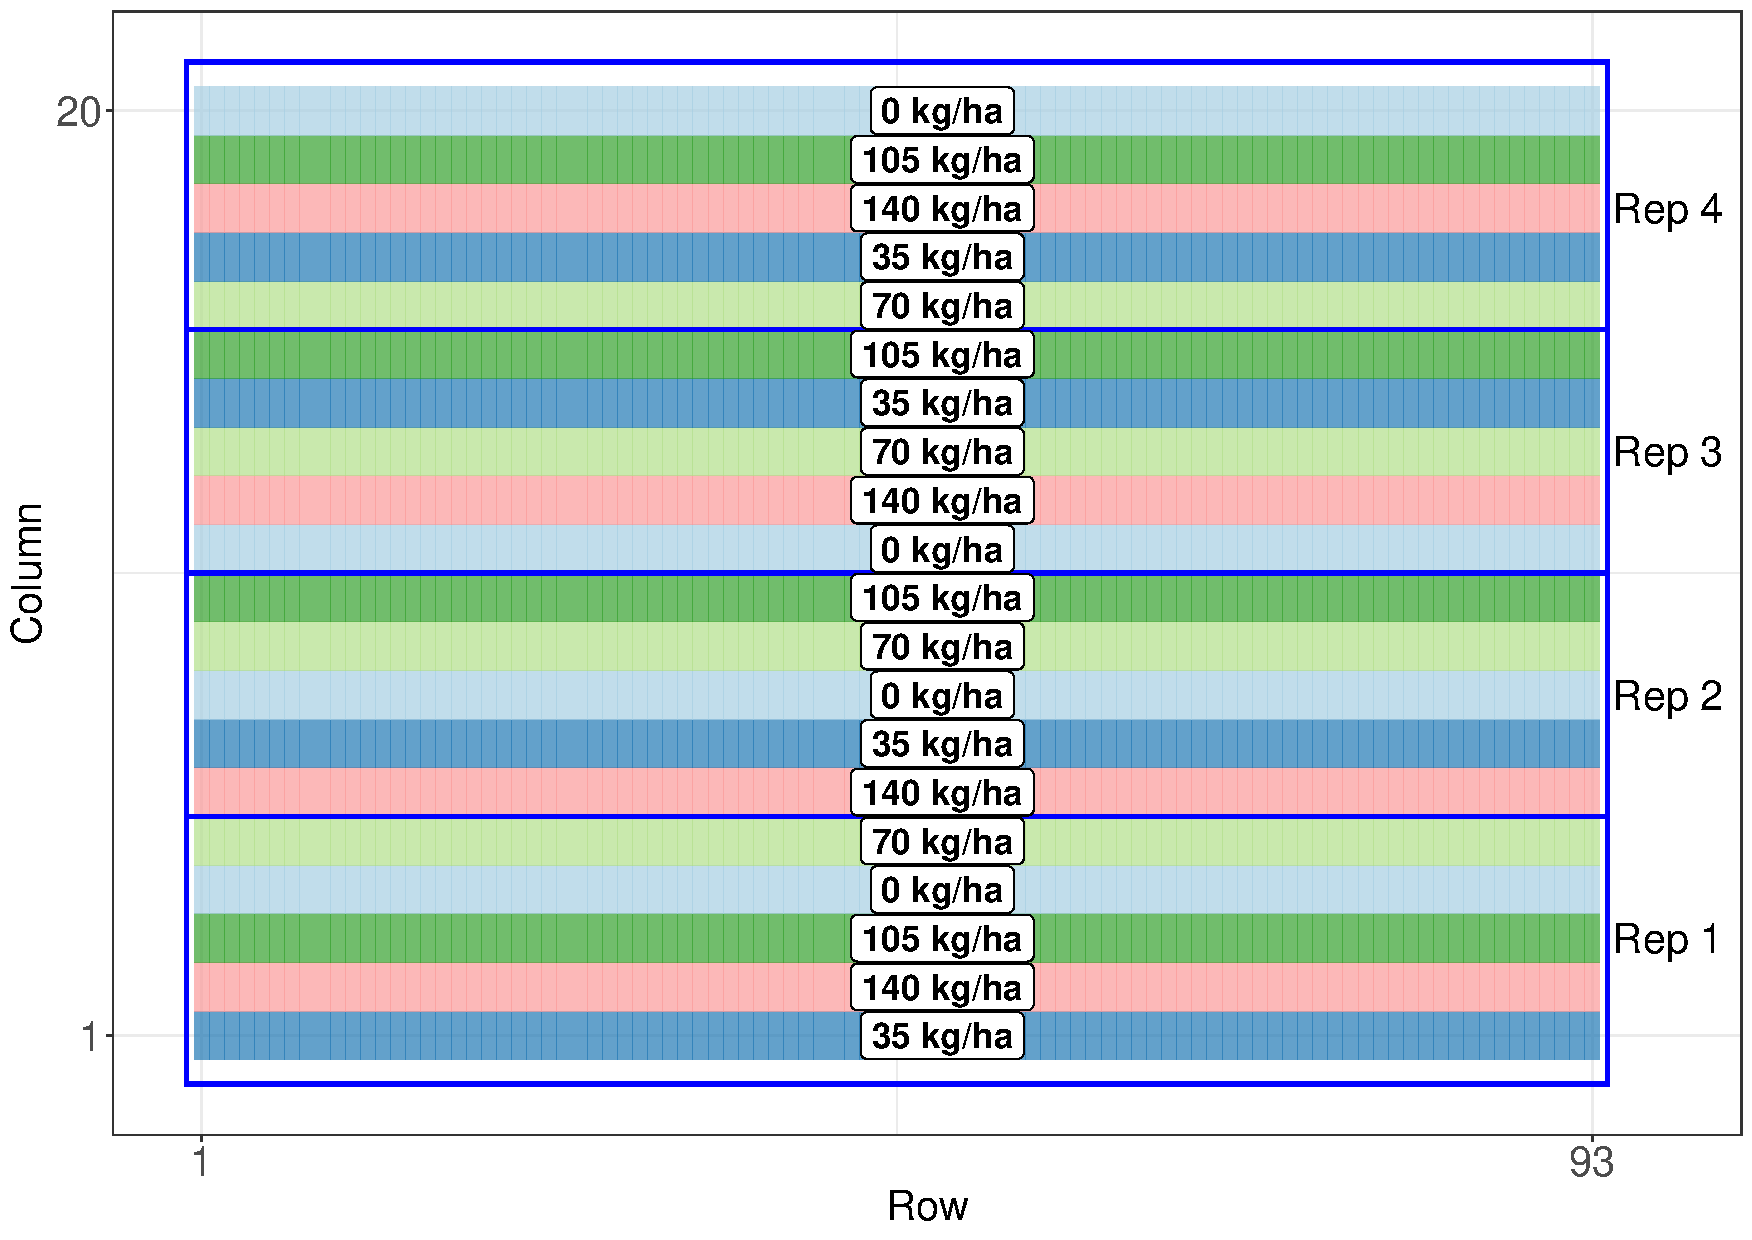
\includegraphics[width=\linewidth]{Col_RandNitro_V4.pdf}
		%\caption{Treatments are randomly allocated into large strips in each replicate block.}\label{fig:RandNitrogen}
	\end{subfigure}
	\hspace{0.05\textwidth}
	\begin{subfigure}[t]{0.45\textwidth}
		\centering
		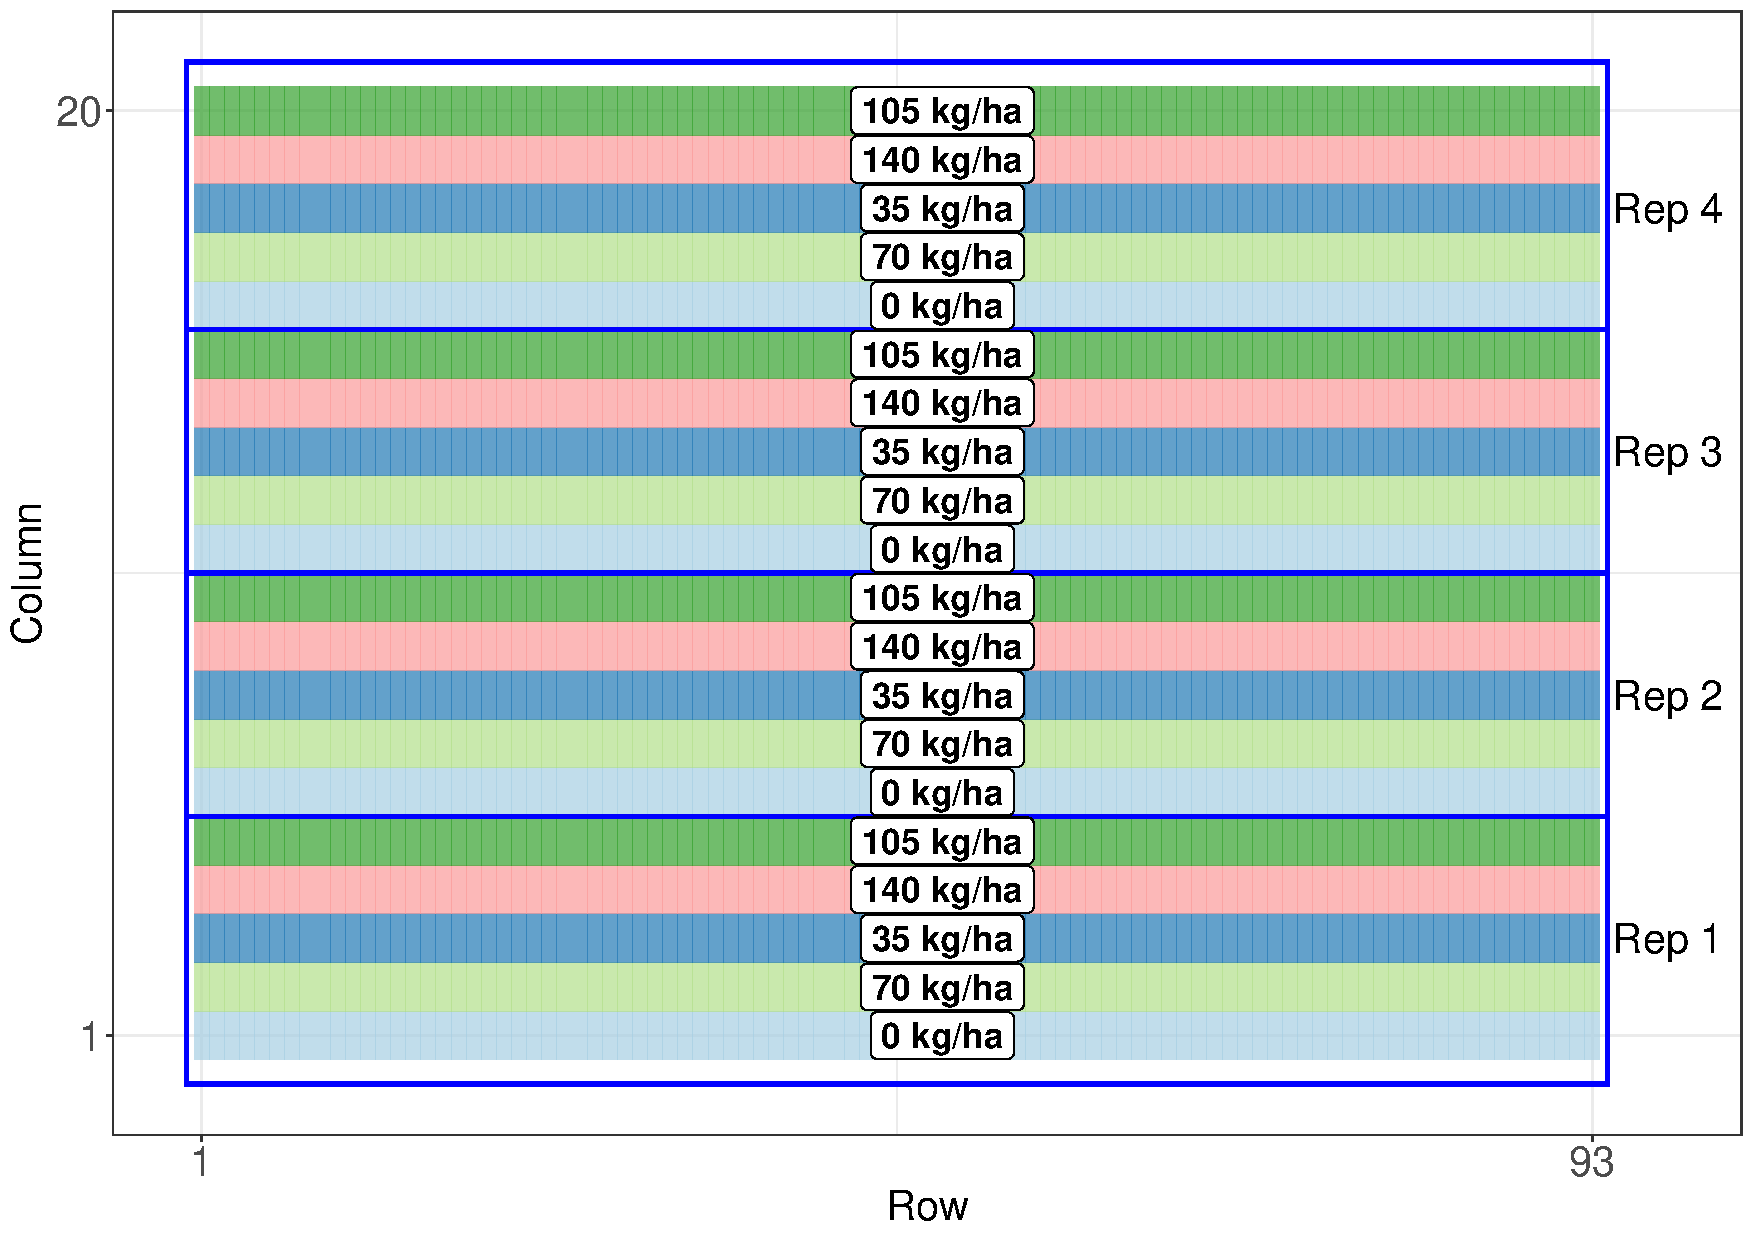
\includegraphics[width=\linewidth]{Col_SystNitro_V4.pdf}
		%\caption{Treatments are systematically allocated into large strips in each replicate block.}\label{fig:SystNitrogen}
	\end{subfigure}
	\caption{\revision{The nitrogen treatments with five levels (0, 35, 70, 105 and 140 kg/ha) randomly (\textit{left}) and systematically (\textit{right}) allocated into strips in each replicate block.}}\label{fig:Nitrogen}
\end{figure}


\zc{We investigate \revision{all possible} combination\revision{s} of the following factors}: \revision{(i)} types of design with two levels, \revision{namely,} randomised and systematic; \revision{(ii)} response relationship with two levels, \revision{namely,} linear and quadratic; \revision{(iii)} correlation coefficients \revision{corresponding to the random effects within each plot} with two levels, \revision{namely,} low and high; \revision{(iv)} spatial variation \revision{between grid points} with three levels, \revision{namely,} identity (no spatial trend), $\AR\otimes\AR$, and \Matern form. \zc{This results in \revision{24} unique combinations. For each combination, we simulated yield data and fitted the GWR model for three bandwidth values of 5, 9 and the optimum \revision{value selected} by AICc.} \revision{For a systematic design in our simulation study, all the treatment levels (five nitrogen levels) can be covered by the bandwidth of 5, making it adequate for inference based on a quadratic response model}. \revision{On the other hand}, the bandwidth of 9 \revision{may be necessary} to cover all possible treatment levels in a randomised design. In particular, if identical treatments are positioned at the far left edge of the first replicate block and \revision{at} the far right edge of the second replicate block, a bandwidth smaller than 9 would  \revision{result in} the GWR model capturing only the treatments between these boundaries, thereby missing the treatment level\revision{s} at the extremes.


\revision{To specify the} linear relationship \revision{in the simulation study}, we \revision{consider the values of $65$ and $0.05$ for the} global intercept $b_0$ and slope $b_1$ coefficients, respectively, \zc{in model \eqref{eq:underlying}}. The variances of \revision{the coefficients} $\bm{u}_i$ are \revision{set to $5$ for $\sigma_{u_0}$ and $0.01$ for $\sigma_{u_1}$}. The\revision{se} parameters are chosen according to the estimates \revision{reported} by \textcite{Cao2022Bayesian}. For the $\AR\otimes\AR$ covariance matrix in \eqref{eq:ar1cov}, the two correlation parameters \revision{$\rho_c$ and $\rho_r$ are set to $0.15$ and $0.50$, respectively}. We \revision{assume} a higher correlation in the row \revision{direction because} the crop is traditionally sown and harvested along \revision{the column direction,} \revision{and} the correlation is higher in the \revision{direction} perpendicular \revision{to the sowing} direction \parencite{Marchant2019Establishinga}. For the \Matern covariance matrix \eqref{eq:matcov}, we set \revision{the value of the variance parameter $\sigma_d^2$ to $1$, the value of the parameter $r$ to $1$, and the value of the parameter $\nu$ to $3/2$}. After drawing samples of $\bm{u}$ from $\N(0,\Sigma_u)$, the spatially varying coefficients \revision{$\bm{\beta}_0$ and $\bm{\beta}_1$ are specified using the relations} $\bm{\beta}_0 = b_0 + \bm{u}_0$ and $\bm{\beta}_1 = b_1 + \bm{u}_1$. 

For the quadratic relationship, we \revision{consider the} \zc{values of $65$, $0.05$ and $-0.0003$ for the coefficients $b_0$, $b_1$, and $b_2$, respectively.} \revision{These choices make the response} curve concave down. \revision{For the variance components,} we \zc{set to $5$ for $\sigma_{u_0}$, $0.01$ for $\sigma_{u_1}$, and $0.0001$ for $\sigma_{u_2}$}. The rest of the parameters \revision{left} unchanged. \revision{Consequently}, the true spatially varying coefficients are $\bm{\beta}_0 = b_0 + \bm{u}_0$, $\bm{\beta}_1 = b_1 + \bm{u}_1$, and $\bm{\beta}_2 = b_2 + \bm{u}_2$ \zc{for the quadratic model}. 

Figure \ref{fig:Lines} illustrates \revision{the global yield response to Nitrogen} for the linear and quadratic relationships.
\begin{figure}[H]
	\begin{subfigure}[t]{0.45\textwidth}
		\centering
		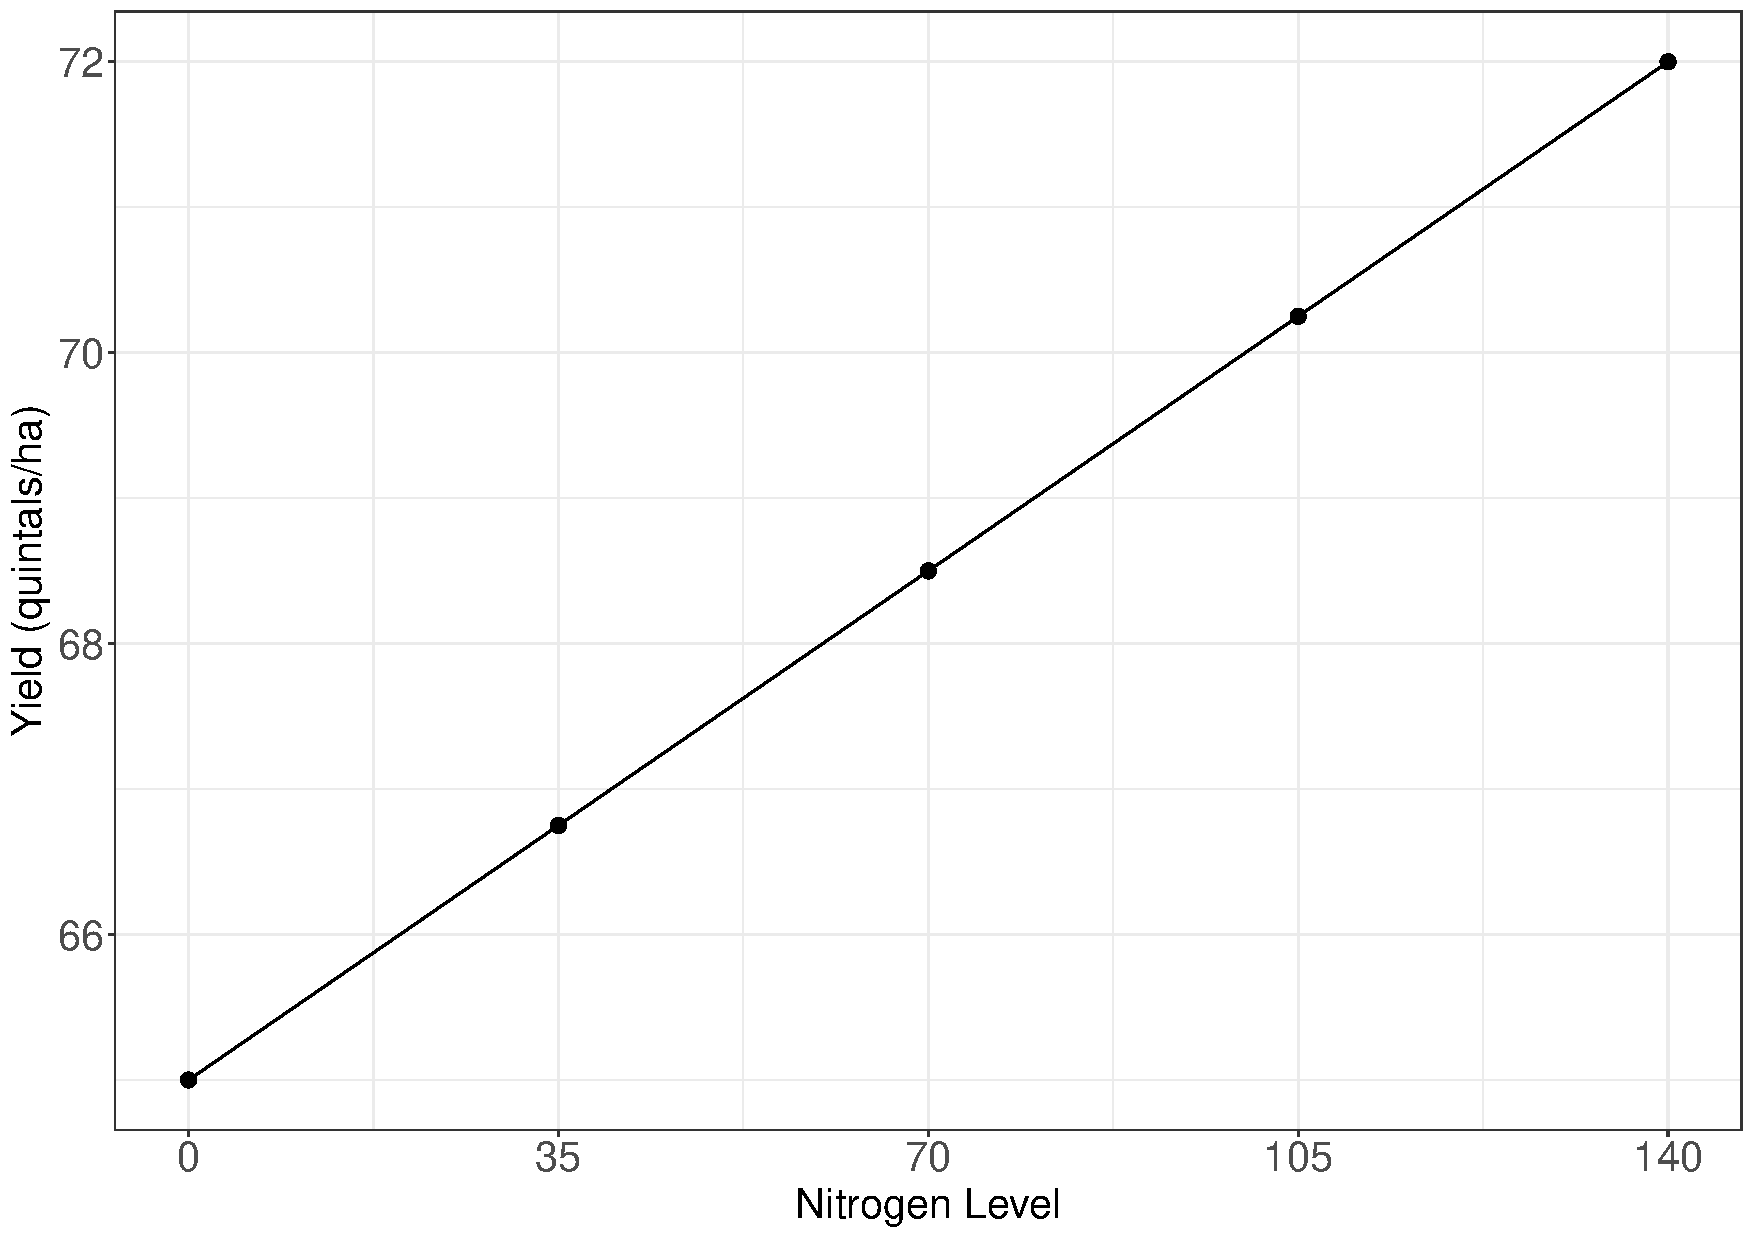
\includegraphics[width=\linewidth]{LinlinesV2.pdf}
		%\caption{}
 \end{subfigure}
	\hspace{0.05\textwidth}
	\begin{subfigure}[t]{0.45\textwidth}
		\centering
		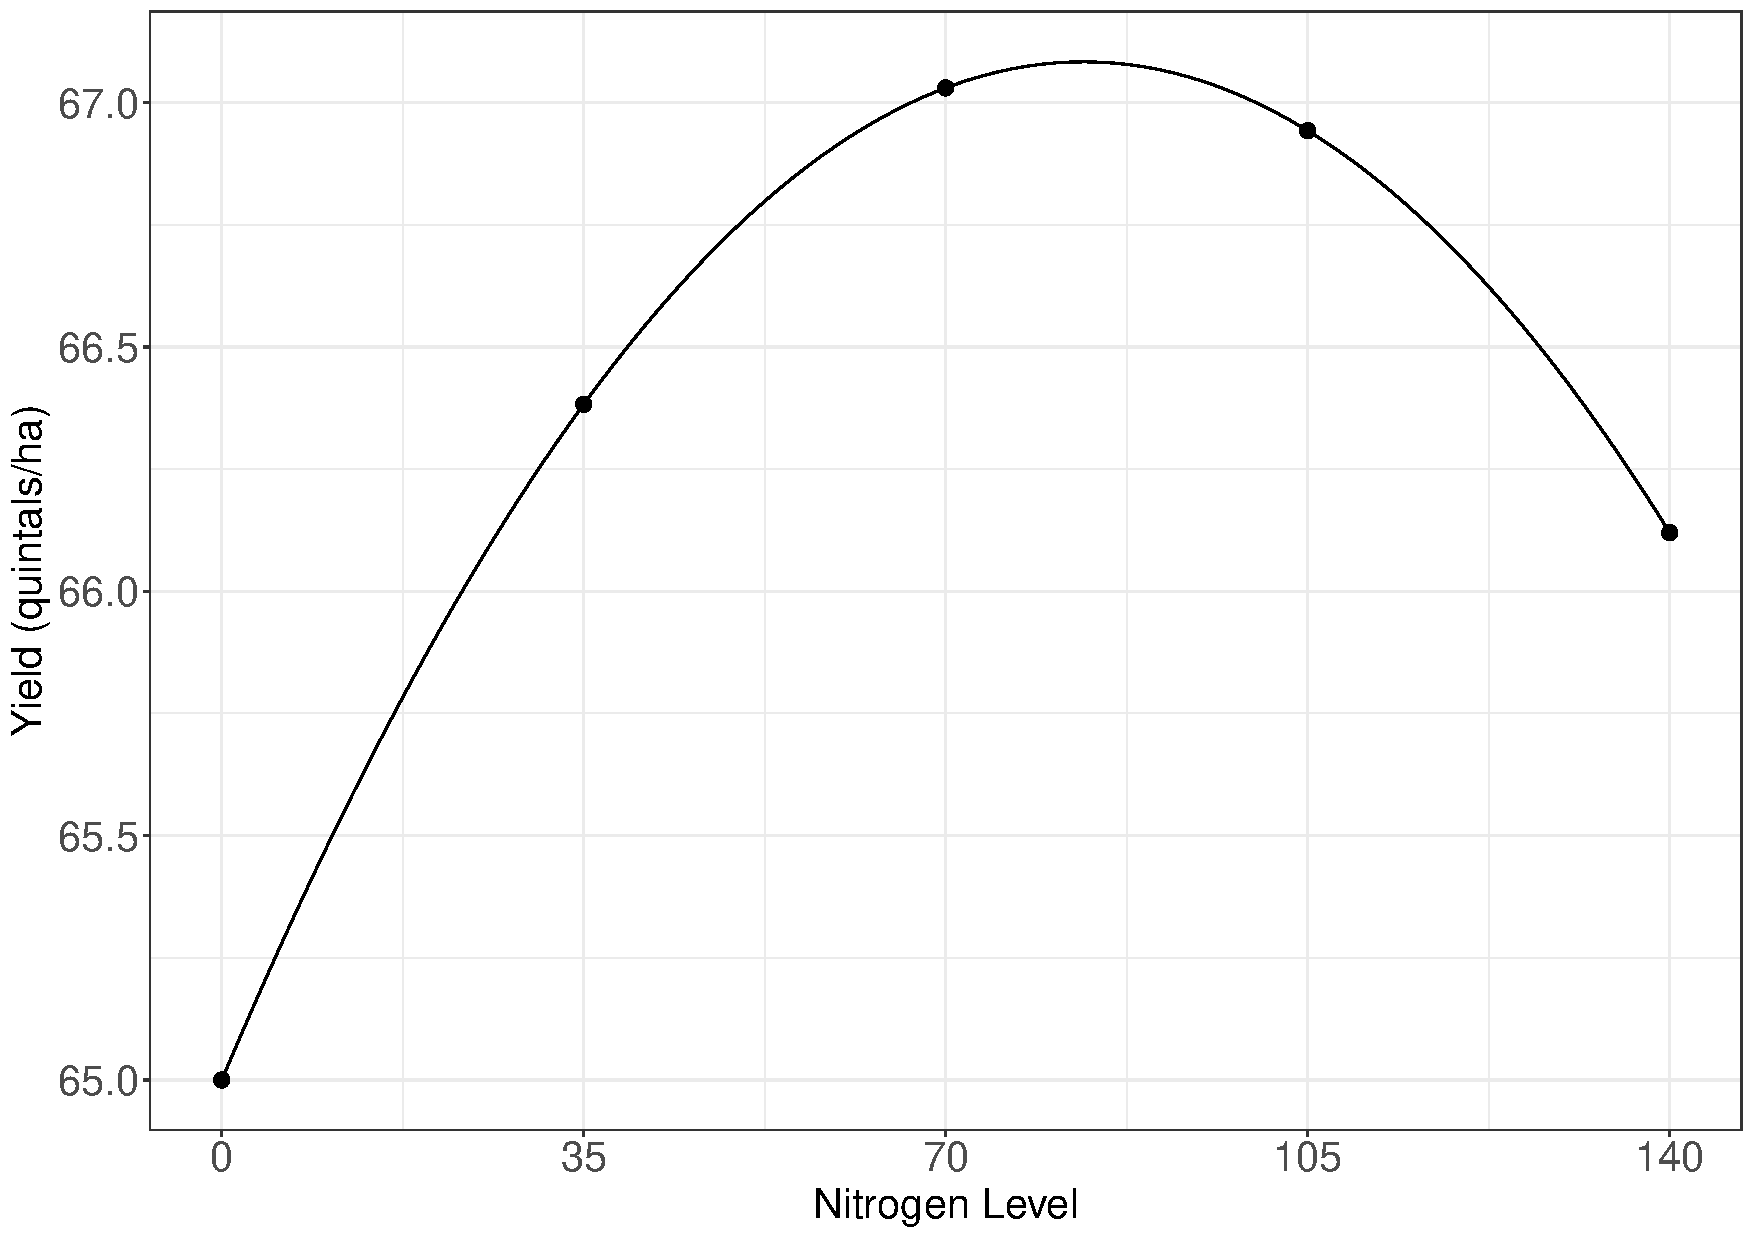
\includegraphics[width=\linewidth]{QualinesV2.pdf}
		%\caption{}
 \end{subfigure}
	\caption{\revision{The global linear relationship of yield and nitrogen is $y=65+0.05N$ (\textit{left}), and the global quadratic relationship between yield and nitrogen is $y=65+0.05N-0.003N^2$ (\textit{right}).}}\label{fig:Lines}
\end{figure}


\zc{To summarise, the} simulated yield \revision{response} is obtained by 
\begin{equation}
\begin{cases}
	\text{Linear}  &y_i = b_0 + u_{0i} + (b_1 + u_{1i})N_i + e_i \\
	\text{Quadratic} &y_i = b_0 + u_{0i} + (b_1 + u_{1i})N_i + (b_2 + u_{2i})N_i^2 + e_i
\end{cases}
\end{equation}
where $N_i$ is the nitrogen rate, $e_i\sim \N(0,1)$ is the error term at grid $i$, $i = 1, \ldots, n$. 



\section{Results}\label{Sec:Res}

\revision{In this section, we assess the performances of randomised and systematic designs in terms of their utility to accurately estimate the model parameters for both linear and quadratic response models. To this end, we perform 1000 simulations of each \revision{of the 24} scenarios\zc{, described} in the previous section.} \zc{In each simulation, we first generate the coefficients for all grids and then apply the treatment in each grid to calculate the yield value using the model coefficients. For the treatment order in each iteration, we randomly picked an order of treatments for a single replicate and repeated this sequence across all other replicates to construct a systematic design. For a randomised design, all replicates have random orders of the treatments.}

% In Section~\ref{Sec:MSE}, the MSEs are compared between the two designs for different \revision{factors, including the choice of} bandwidth, parameter correlation, and spatial covariance matrix. % Section~\ref{Sec:anova} uses \revision{the} analysis of variance (ANOVA) to  \revision{assess} the significance of the factors \revision{considered} in the simulation \revision{study}. %\st{subsection} Section~\ref{Sec:bandselect} \st{states} \revision{presents} the \st{performance of} \revision{results of} bandwidth selection using AICc. 

%By running the simulation 100 times, 

\subsection{\revision{Comparison based on} mean squared errors}\label{Sec:MSE}

% \revision{To assess the performance of different designs for a simulation scenario,} we \revision{computed the} mean squared error (MSE) \revision{corresponding to all} coefficient \revision{estimates}. This was \revision{computed} by \revision{taking} the difference of true coefficients $\bm{\beta}$ (i.e., $b + \bm{u}$) and the estimated spatially varying coefficients $\bm{\hat{\beta}}$ (i.e., $\hat{b} + \bm{\hat{u}}$) for each grid, and then \revision{averaging} the squared discrepancies across \revision{all the grid points in} the field.

\revision{Figures~\ref{fig:LinBetaMSE} and \ref{fig:LinBetaMSEeta01} show the results of linear models for the cases of low ($\epsilon = 1$) and high ($\epsilon = 0.1$) correlations, respectively, while Figures~\ref{fig:QuadBetaMSE} and \ref{fig:QuadBetaMSEeta01} show the results of quadratic models for the same low and high correlations, respectively. To specify the covariance matrix $V_s$ used in producing the results in these figures, we use the following labels: (i) ``NS'' for the identity matrix representing no spatial correlation, (ii) ``AR1'' for $\AR(0.15)\otimes \AR(0.5)$, and (iii) ``Matern'' for \Matern covariance with $\nu=3/2$.} \zc{Note that the model parameters and their corresponding MSEs are small values, and this makes it difficult to compare the MSEs of different scenarios using the original scale of MSE values. Therefore, to enhance clarity in visualisation and comparison, we have multiplied the MSEs of $\bm{\beta}_1$ and $\bm{\beta}_2$ by $10^4$ and $10^8$, respectively, in the figures presented below. }



% Paragraph about Figure 3 and the performance for a linear response
\revision{For} the linear response model, both randomised and systematic designs perform similarly\revision{, particularly for the case NS.} Figure~\ref{fig:LinBetaMSE} shows that the MSE \revision{corresponding to} $\zc{\hat{\bm{\beta}}}_0$ for all bandwidths \revision{are fairly similar for both} designs \zc{without spatial correlation}. \zc{However, when a spatial covariance matrix is incorporated in the model, the MSE results, presented also in Tables \ref{tb:MSElinear} and \ref{tb:MSElinearHigh}, in the figures below show that the MSE medians corresponding to $\hat{\bm{\beta}}_1$ for $\AR\otimes\AR$ and \Matern cases are lower for the systematic design.} 
%This is true regardless of \revision{the correlation within grids considered in a simulation}, small ($\epsilon=1$) or high ($\epsilon=0.1$) as is shown in Figure \ref{fig:LinBetaMSEeta01}. %% The GWR with bandwidth selected by AICc has a smaller MSE for its coefficients than the model with a fixed bandwidth (Figure \ref{fig:LinBetaMSE}). 


\begin{figure}[!htp]
	\centering
	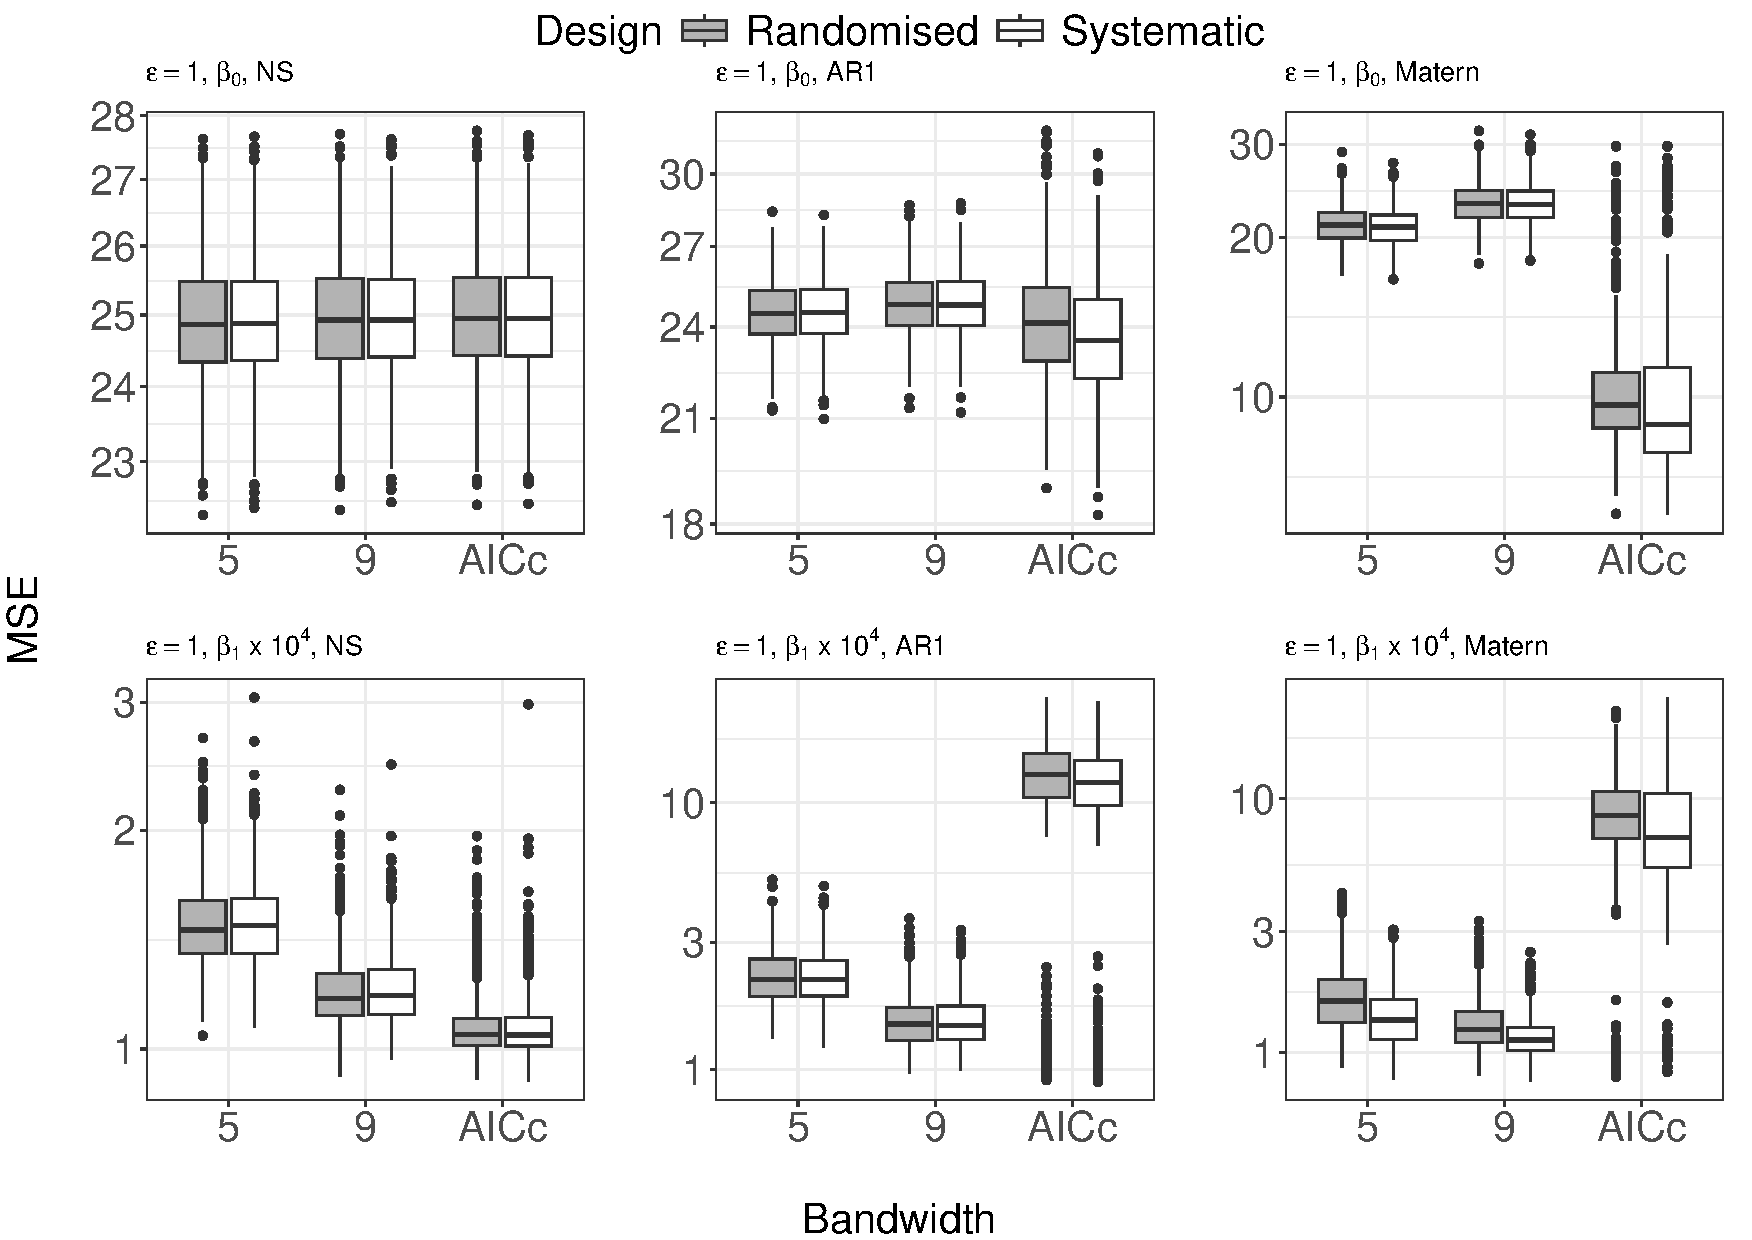
\includegraphics[width=\linewidth]{Col_LinCombMSE_newpar_1K_V4.pdf}
	\caption{\zc{Boxplots of MSE for $\zc{\hat{\bm{\beta}}}_0$ and $\zc{\hat{\bm{\beta}}}_1$ in GWR models using different bandwidths for the simulated data with a linear response. The simulated data had different spatial covariance matrices (NS, AR1$\otimes$AR1 and \Matern) and a low correlation between the parameters ($\epsilon=1$).}}\label{fig:LinBetaMSE}
\end{figure}


\begin{figure}[!thp]
	\centering
	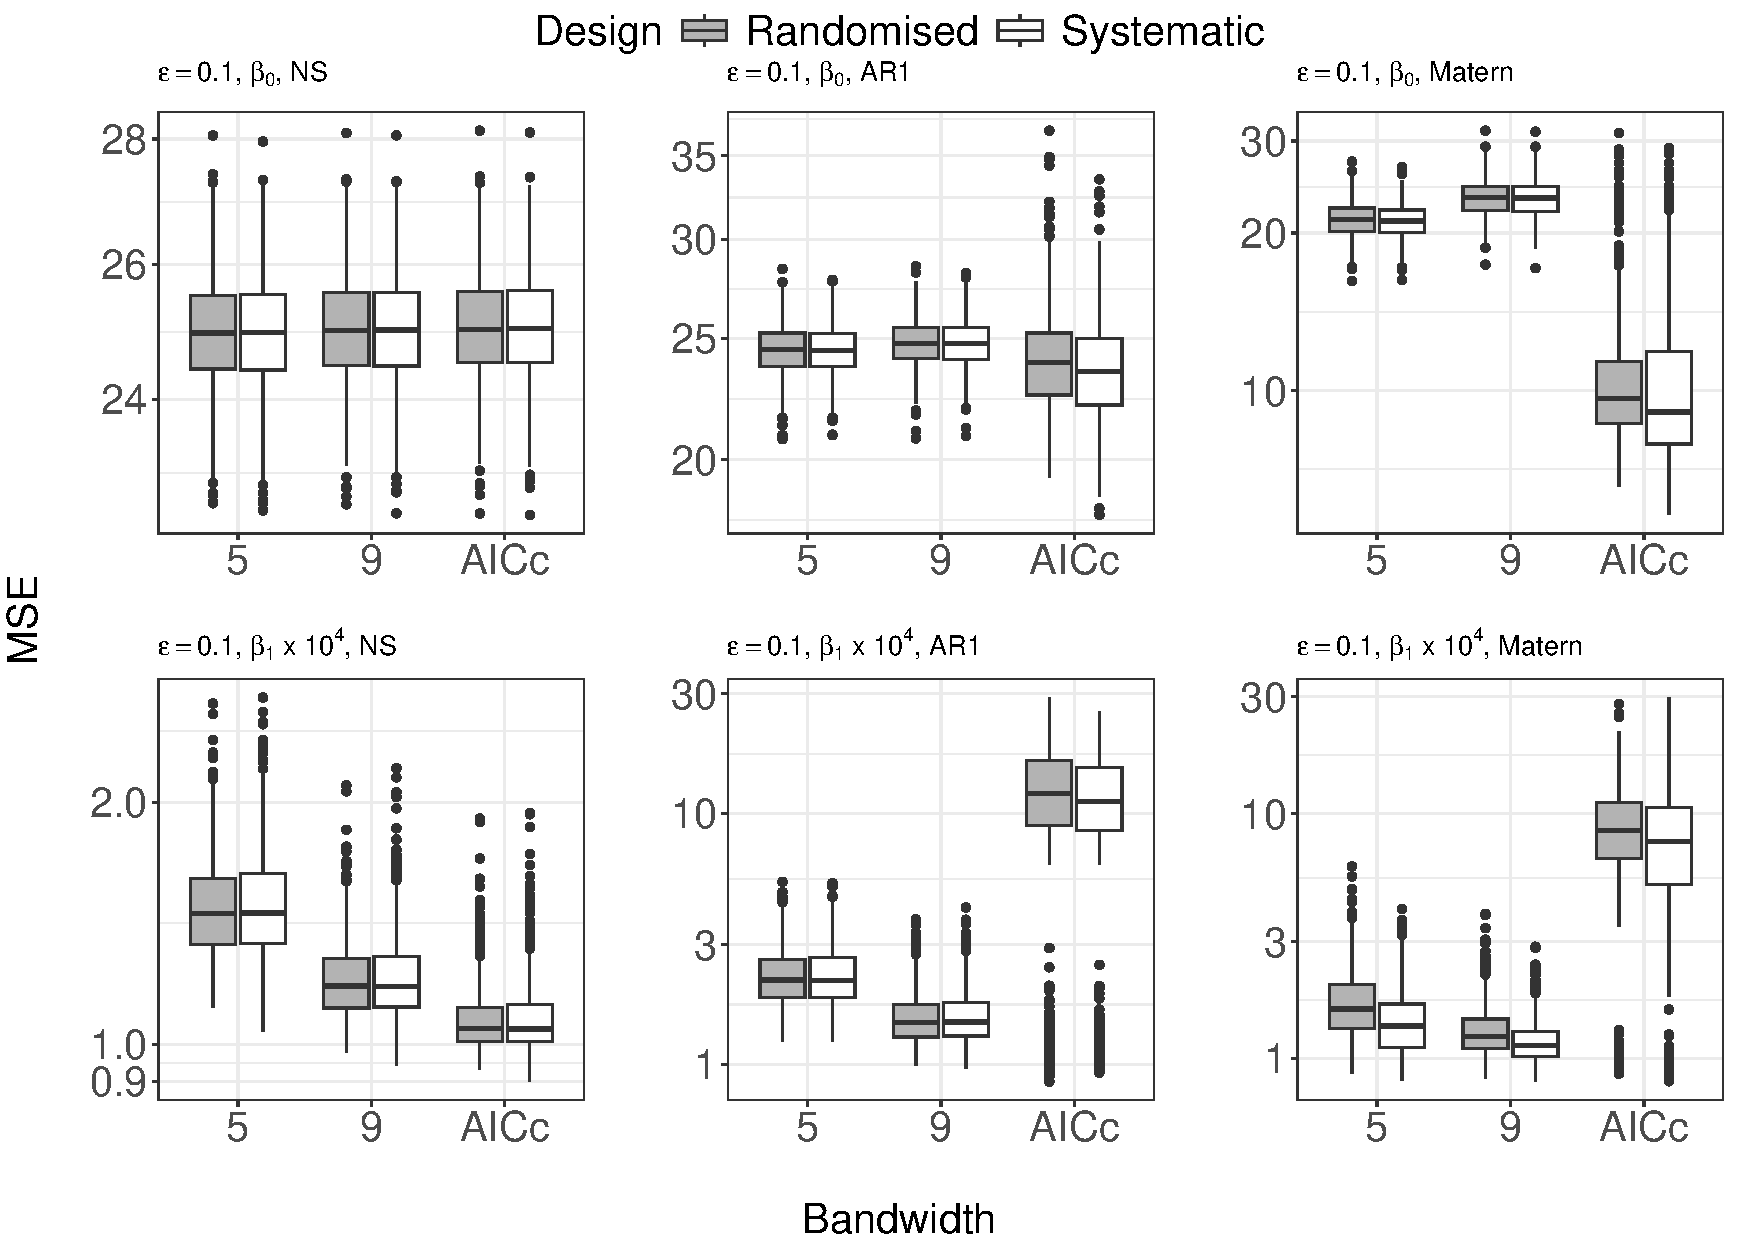
\includegraphics[width=\linewidth]{Col_LinCombMSE_newpar_1K_eta01_V4.pdf}
	\caption{\zc{Boxplots of MSE for $\zc{\hat{\bm{\beta}}}_0$ and $\zc{\hat{\bm{\beta}}}_1$ in GWR models using different bandwidths for the simulated data with a linear response. The simulated data had different spatial covariance matrices (NS, AR1$\otimes$AR1 and \Matern) and a high correlation between the parameters ($\epsilon=0.1$).}}\label{fig:LinBetaMSEeta01}
\end{figure}




% Paragraph about Figure 4 and the performance for a linear response
\revision{For} the quadratic response \revision{model}, Figures \ref{fig:QuadBetaMSE} and \ref{fig:QuadBetaMSEeta01} show that the GWR estimates \revision{of both ${\bm{\beta}}_{1}$ and ${\bm{\beta}}_{2}$ based on fixed bandwidths of $5$ and $9$ for systematic designs outperform the estimates obtained for randomised designs when spatial correlation (``AR1'' and ``Matern") is present in yield data}. \revision{Using the AICc optimal bandwidth, GWR successfully estimates the intercepts $\zc{\bm{\beta}_0}$ but fails to accurately estimate} \zc{linear and quadratic} coefficients $\zc{\bm{\beta}}_1$ and $\zc{\bm{\beta}}_2$, \revision{resulting in MSEs that are relatively larger than those obtained using a fixed bandwidth}. \revision{Overall, the results of our simulation study indicate that the systematic designs are superior to randomised designs in enabling accurate and precise estimation of spatially varying treatment effects, especially when the response model is a quadratic function of the treatment levels.} 



%If we only compare across two types of designs, it proves that \zc{fitting} GWR to a systematic design \zc{is more robust} than \zc{fitting it to} a randomised design if the assumption is a quadratic response.

\begin{figure}[!thp]
	\centering
	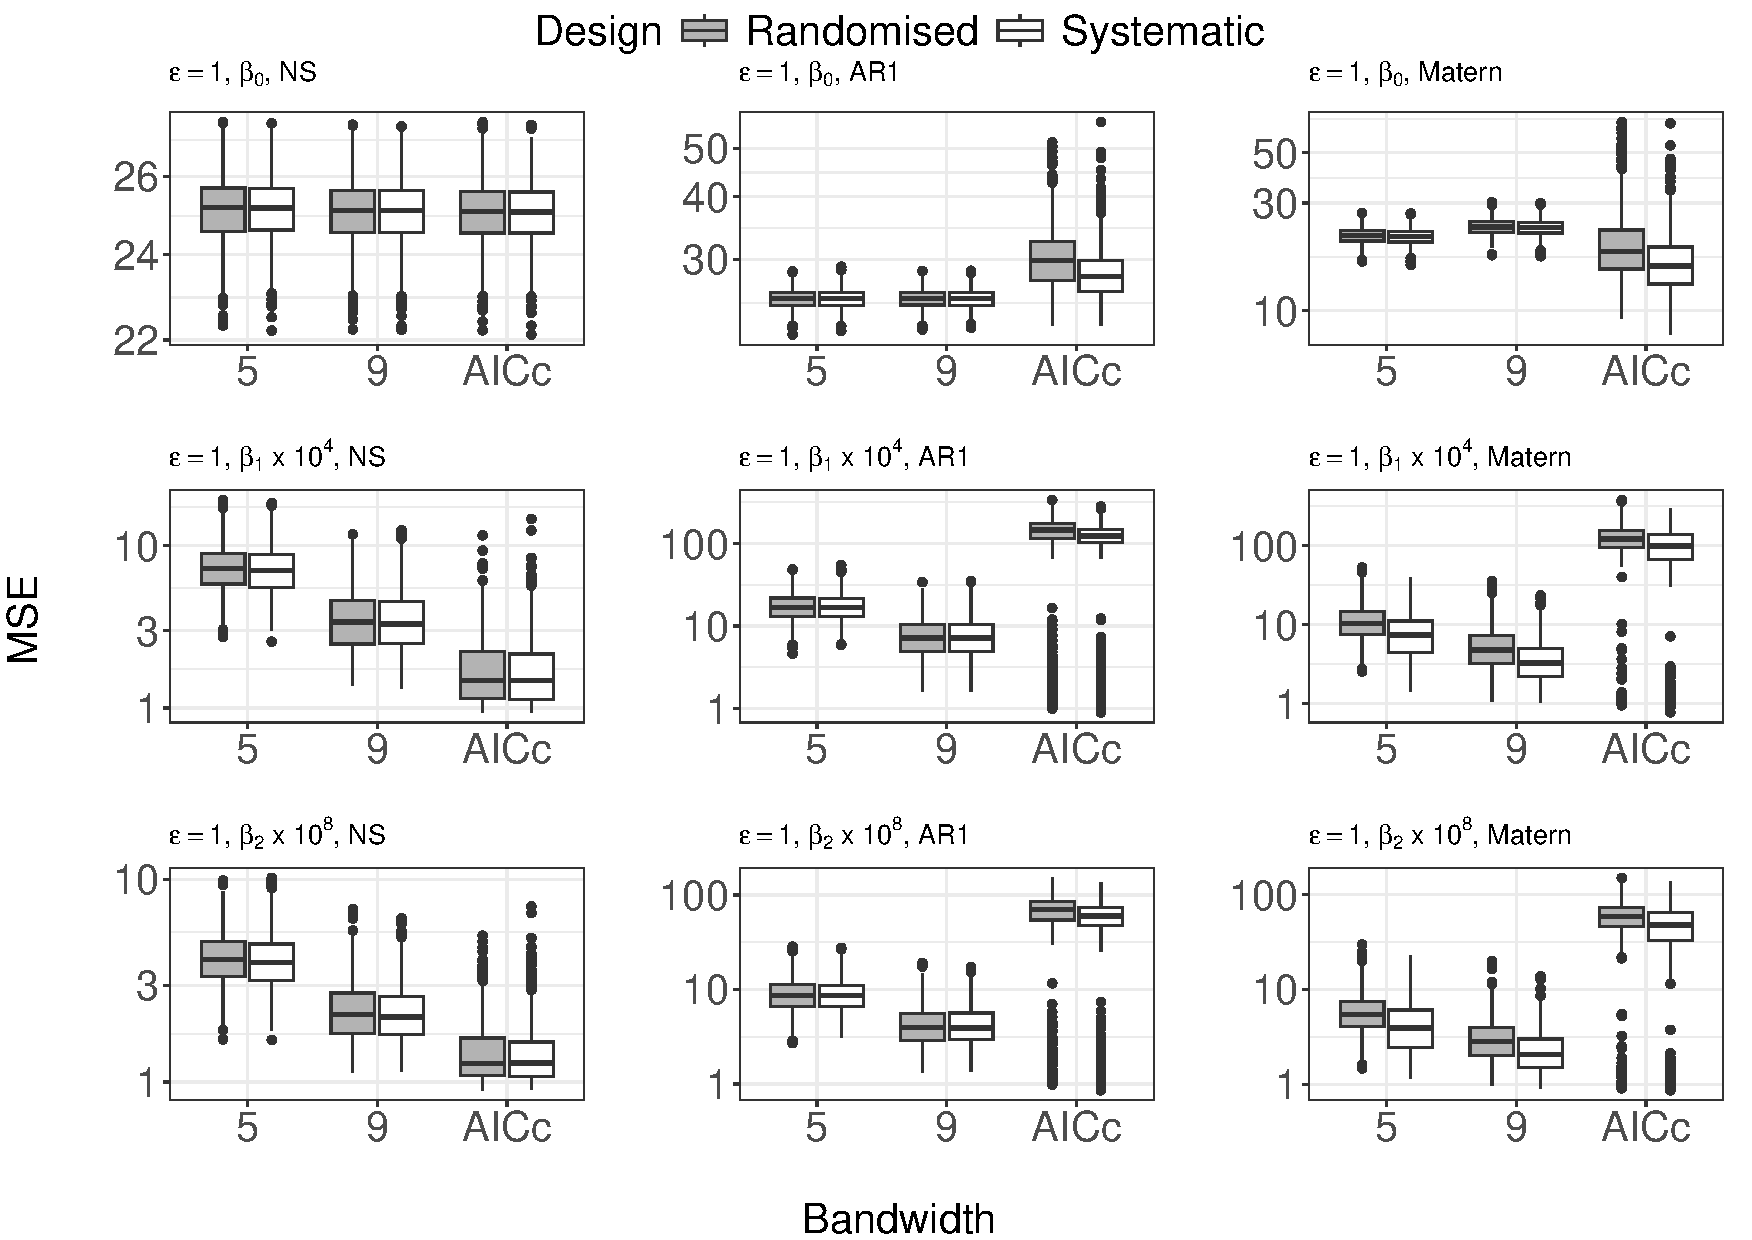
\includegraphics[width=\linewidth]{Col_QuaCombMSE_newpar_1K_V4.pdf}
	\caption{\zc{Boxplots of MSE for $\zc{\hat{\bm{\beta}}}_0$, $\zc{\hat{\bm{\beta}}}_1$ and $\zc{\hat{\bm{\beta}}}_2$ in GWR models using different bandwidths for the simulated data with a quadratic response. The simulated data had different spatial covariance matrices (NS, AR1$\otimes$AR1 and \Matern) and a low correlation amongst the parameters ($\epsilon=1$).}} \label{fig:QuadBetaMSE}
\end{figure}


\begin{figure}[!thp]
	\centering
	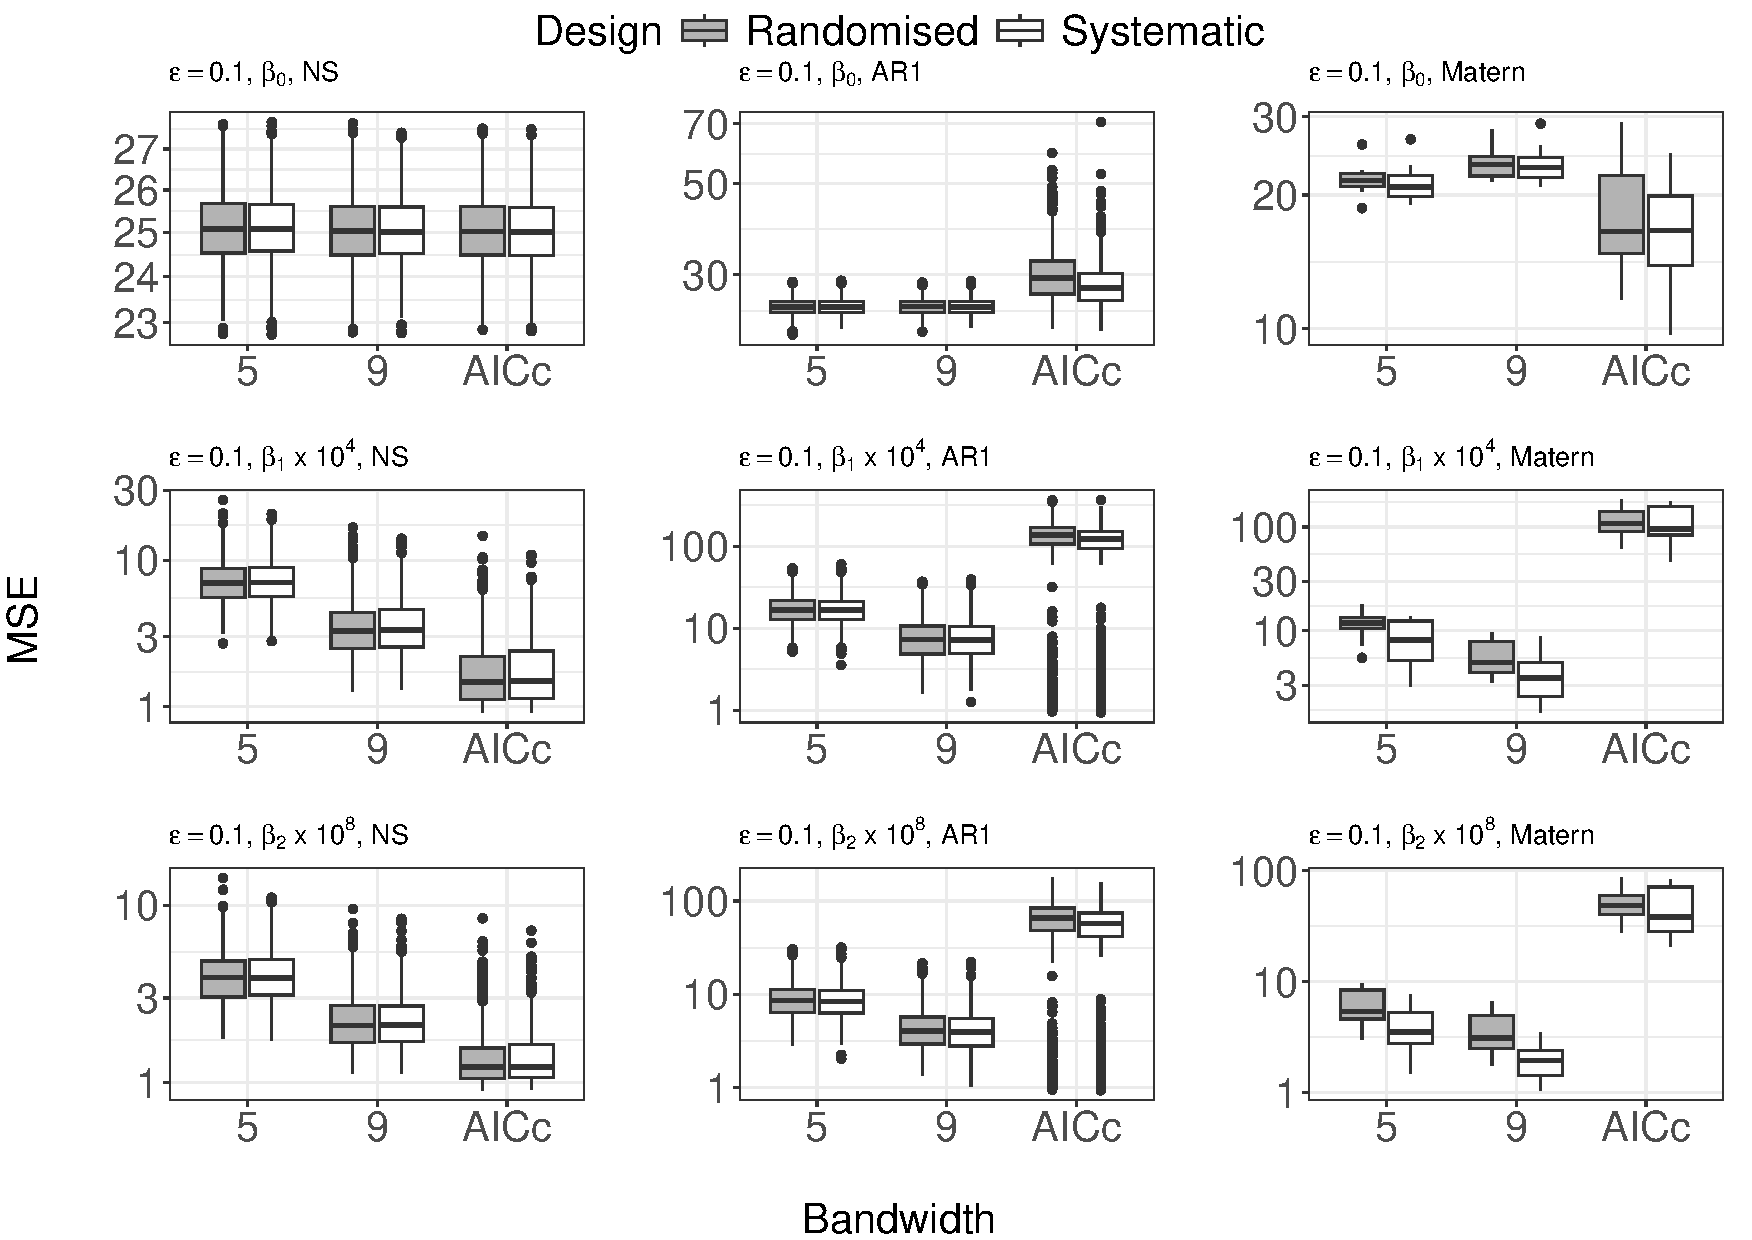
\includegraphics[width=\linewidth]{Col_QuaCombMSE_newpar_1K_eta01_V4.pdf}
	\caption{\zc{Boxplots of MSE for $\zc{\hat{\bm{\beta}}}_0$, $\zc{\hat{\bm{\beta}}}_1$ and $\zc{\hat{\bm{\beta}}}_2$ in GWR models using different bandwidths for the simulated data with a quadratic response. The simulated data had different spatial covariance matrices (NS, AR1$\otimes$AR1 and \Matern) and a high correlation amongst the parameters ($\epsilon=0.1$).}} \label{fig:QuadBetaMSEeta01}
\end{figure}
% Bandwidth MSE Result

%%The relative MSE for each bandwidth was found to change according to the spatial covariance matrix as well as the coefficient. When no spatial variation was simulated for $\beta_1$ and $\beta_2$, the AICc-selected bandwidth has the lowest MSE, followed by the fixed bandwidths of 9 and then 5. When there is spatial variation (either AR1$\otimes$AR1 or \Matern) present the estimation for $\beta_1$ and $\beta_2$ has the lowest MSE when using bandwidth 9, followed by 5 and then bandwidth from AICc. The intercept ($\beta_0$) shows only significant changes in MSE amongst the bandwidths when the \Matern spatial covariance was considered. In this case, the bandwidth selected by AICc produces the smallest MSE.

\revision{Moreover,} MSE \zc{comparisons} reveal that the choice of bandwidth \zc{may influence} the relative performance \revision{of the two designs differently depending on whether the intercept coefficient or the slope coefficients are being estimated. Differences in relative performance are also observed for different forms of spatial covariance matrices considered in the simulation scenarios.}  In scenarios without spatial variation, \revision{when estimating} \zc{$\zc{\bm{\beta}}_0$}, $\zc{\bm{\beta}}_1$ and $\zc{\bm{\beta}}_2$, the AICc-selected bandwidths \revision{produce} \zc{the lowest} MSE \revision{medians}. \zc{In contrast, when} spatial variation \zc{is} present (utilising either AR1$\otimes$AR1 or \Matern covariance structures), the bandwidth of 9 consistently produces the most accurate estimates of $\zc{\bm{\beta}}_1$ and $\zc{\bm{\beta}}_2$, outperforming the \revision{estimates obtained using either the} bandwidth of 5 or the one chosen by AICc. %% Notably, for the intercept ($\zc{\bm{\beta}}_0$), significant changes in MSE amongst the bandwidths \zc{are} observed only in the context of the \Matern spatial covariance. 
% Here, the bandwidth selected by AICc resulted in the smallest MSE, highlighting its efficacy when dealing with spatially correlated residuals following the \Matern covariance structure. 

Tables \ref{tb:MSElinear} and \ref{tb:MSElinearHigh} \revision{present} the median MSEs \revision{corresponding to the parameter estimation for} the linear response \revision{model in the} two scenarios \revision{of low ($\epsilon=1$) and high ($\epsilon= 0.1$) correlations, respectively}.

% \begin{table}[!htp]
% 	\centering
% \begin{threeparttable}
% 	\caption{\zc{Median MSE of GWR coefficient estimates for a linear response when the correlation between the parameters is low ($\epsilon=1$).}}\label{tb:MSElinear}
% 	\begin{tabular}{llcccccc}
% 		\toprule
% 		&  & \multicolumn{3}{c}{Randomised Design} & \multicolumn{3}{c}{Systematic Design} \\ \midrule
%   	\multirow{2}{*}{$V_s$ with $\epsilon=1$} & \multirow{2}{*}{Coefficients}  & \multicolumn{6}{c}{Bandwidth}\\ 
% 		&  & 5  & 9  & AICc & 5  & 9  & AICc \\ \midrule
% 		\multirow{2}{*}{NS}   & $\zc{\hat{\bm{\beta}}}_0$ & 24.852 &	24.933 &	24.912&	\bf{24.781}\tnote{$\dagger$} &	24.850 &	24.861 \\ 
% 		& $\zc{\hat{\bm{\beta}}}_1 (\times 10^4)$ & 1.683 &	1.341 &	1.398 &	1.615 &	\bf{1.320}\tnote{$\dagger$} &	1.361 \\  \midrule
%  \multirow{2}{*}{AR1$\otimes$AR1}  & $\zc{\hat{\bm{\beta}}}_0$ & 24.401 &	24.649 &	23.695 &	24.295 &	24.684 &	\bf{23.118}\tnote{$\dagger$} \\ 
% 		& $\zc{\hat{\bm{\beta}}}_1 (\times 10^4)$ & 2.489 &	1.790 &	10.071 &	2.441 &	\bf{1.740}\tnote{$\dagger$} &	9.995 \\ \midrule
% 		\multirow{2}{*}{\Matern} & $\zc{\hat{\bm{\beta}}}_0$ & 20.482 &	22.432 &	9.801 &	20.319 &	22.194 &	\bf{9.280}\tnote{$\dagger$} \\ 
% 		& $\zc{\hat{\bm{\beta}}}_1 (\times 10^4)$ & 1.683 &	1.378 &	8.049 &	1.398 &	\bf{1.197}\tnote{$\dagger$} &	7.022 \\
% 		\bottomrule
% 	\end{tabular}
% 	\begin{tablenotes}
% 	\item[$\dagger$] \footnotesize Indicates the smallest MSE for the row.
% 	\end{tablenotes}
% \end{threeparttable}
% \end{table}


\begin{table}[!htp]
\centering
\begin{threeparttable}
\caption{\zc{Median MSE of GWR coefficient estimates for a linear response when the correlation between the parameters is low ($\epsilon=1$).}}\label{tb:MSElinear}
\begin{tabular}{ll|ccc|ccc}
\toprule
\multicolumn{2}{c}{Linear Response with $\epsilon=1$} & \multicolumn{3}{c}{Randomised Design} & \multicolumn{3}{c}{Systematic Design} \\ \midrule
\multirow{2}{*}{$V_s$} & \multirow{2}{*}{Coefficients}  & \multicolumn{6}{c}{Bandwidth}\\ 
&  & 5  & 9  & AICc & 5  & 9  & AICc \\ \midrule
\multirow{2}{*}{NS} & $\zc{\hat{\bm{\beta}}}_0$ & \bf{24.868}\tnote{$\dagger$}  & 24.927   & 24.952   & 24.883     & 24.931     & 24.953 \\
  &$\zc{\hat{\bm{\beta}}}_1 (\times 10^4)$ & 1.458   & 1.175   & 1.048 & 1.479    & 1.185   & \bf{1.045}\tnote{$\dagger$}   \\ \midrule
\multirow{2}{*}{AR1}& $\zc{\hat{\bm{\beta}}}_0$ & 24.471  & 24.807   & 24.134   & 24.513      & 24.788    & \bf{23.538}\tnote{$\dagger$}  \\
     & $\zc{\hat{\bm{\beta}}}_1 (\times 10^4)$ & 2.178   & 1.484    & 12.744     & 2.173    & \bf{1.463}\tnote{$\dagger$}     & 11.922  \\ \midrule
\multirow{2}{*}{Matern} & $\zc{\hat{\bm{\beta}}}_0$ & 21.125  & 23.215   & 9.667      & 20.928     & 23.100    & \bf{8.871}\tnote{$\dagger$} \\
      & $\zc{\hat{\bm{\beta}}}_1 (\times 10^4)$& 1.600   & 1.232    & 8.591      & 1.343     & \bf{1.123}\tnote{$\dagger$}  & 7.030   \\ 
\bottomrule
\end{tabular}
\begin{tablenotes}
\item[$\dagger$] \footnotesize Indicates the smallest MSE for the row.
\end{tablenotes}
\end{threeparttable}
\end{table}





% \begin{table}[!htp]
% 	\centering
% \begin{threeparttable}
% 	\caption{\zc{Median MSE of GWR coefficient estimates of linear response when the correlation between the parameters is high ($\epsilon=0.1$).} \revision{NOTE: to be updated} }\label{tb:MSElinearHigh}
% 	\begin{tabular}{llcccccc}
% 		\toprule
% 		&  & \multicolumn{3}{c}{Randomised Design} & \multicolumn{3}{c}{Systematic Design} \\ \midrule
%   	\multirow{2}{*}{$V_s$ with $\epsilon=0.1$} & \multirow{2}{*}{Coefficients}  & \multicolumn{6}{c}{Bandwidth}\\ 
% 		&  & 5  & 9  & AICc & 5  & 9  & AICc \\ \midrule
% 		\multirow{2}{*}{NS}   & $\zc{\hat{\bm{\beta}}}_0$ & 24.808 &	24.925 &	24.927&	\bf{24.761}\tnote{$\dagger$}  &	24.824 &	24.837 \\ 
% 		& $\zc{\hat{\bm{\beta}}}_1 (\times 10^4)$ & 1.623 &	1.334 &	1.382 &	1.590 &	\bf{1.304}\tnote{$\dagger$}  &	1.352 \\  \midrule
% 		\multirow{2}{*}{AR1$\otimes$AR1}  & $\zc{\hat{\bm{\beta}}}_0$ & 24.379 &	24.690 &	23.650 &	24.321  &	24.633 &	\bf{23.416}\tnote{$\dagger$} \\ 
% 		& $\zc{\hat{\bm{\beta}}}_1 (\times 10^4)$ & 2.343 &	\bf{1.683}\tnote{$\dagger$}  &	9.889 &	2.372 &	1.691 &	9.409 \\ \midrule
% 		\multirow{2}{*}{\Matern} & $\zc{\hat{\bm{\beta}}}_0$ & 20.221 &	21.835 &	9.852 &	19.863 &	21.667 &	\bf{9.383}\tnote{$\dagger$}  \\ 
% 		& $\zc{\hat{\bm{\beta}}}_1 (\times 10^4)$ & 1.731 &	1.390 &	8.109 &	1.422 &	\bf{1.204}\tnote{$\dagger$}  &	7.013 \\
% 		\bottomrule
% 	\end{tabular}
% 	\begin{tablenotes}
% 	\item[$\dagger$] \footnotesize Indicates the smallest MSE for the row.
% 	\end{tablenotes}
% \end{threeparttable}
% \end{table}


\begin{table}[!htp]
	\centering
\begin{threeparttable}
\caption{\zc{Median MSE of GWR coefficient estimates of linear response when the correlation between the parameters is high ($\epsilon=0.1$).}}\label{tb:MSElinearHigh}
\begin{tabular}{ll|ccc|ccc}
\toprule
\multicolumn{2}{c}{Linear Response with $\epsilon=0.1$} & \multicolumn{3}{c}{Randomised Design} & \multicolumn{3}{c}{Systematic Design} \\ \midrule
\multirow{2}{*}{$V_s$} & \multirow{2}{*}{Coefficients}  & \multicolumn{6}{c}{Bandwidth}\\ 
&  & 5  & 9  & AICc & 5  & 9  & AICc \\ \midrule
\multirow{2}{*}{NS}   & $\zc{\hat{\bm{\beta}}}_0$ & \bf{24.964}\tnote{$\dagger$}  & 25.000 & 25.018    & 24.970 & 25.006 & 25.031 \\ 
& $\zc{\hat{\bm{\beta}}}_1 (\times 10^4)$ &  1.455  & 1.181  & 1.047     & 1.456  & 1.180  & \bf{1.044}\tnote{$\dagger$}   \\  \midrule
\multirow{2}{*}{AR1$\otimes$AR1}  & $\zc{\hat{\bm{\beta}}}_0$ & 24.490 & 24.773 & 23.928    & 24.457 & 24.780 & \bf{23.524}\tnote{$\dagger$}    \\ 
& $\zc{\hat{\bm{\beta}}}_1 (\times 10^4)$ &  2.168  & \bf{1.464}\tnote{$\dagger$}  & 12.014    & 2.159  & 1.472  & 11.153    \\ \midrule
\multirow{2}{*}{\Matern} & $\zc{\hat{\bm{\beta}}}_0$ & 21.247 & 23.376 & 9.668     & 21.100 & 23.330 & \bf{9.093}\tnote{$\dagger$}  \\ 
& $\zc{\hat{\bm{\beta}}}_1 (\times 10^4)$ & 1.596 & 1.233  & 8.518     & 1.359  & \bf{1.129}\tnote{$\dagger$}  & 7.676 \\
\bottomrule
\end{tabular}
\begin{tablenotes}
\item[$\dagger$] \footnotesize Indicates the smallest MSE for the row.
\end{tablenotes}
\end{threeparttable}
\end{table}

Tables \ref{tb:MSEquadratic} and \ref{tb:MSEquadraticHigh} \revision{present} the median MSEs \revision{corresponding to the estimation of} quadratic response models for the two scenarios \revision{of low ($\epsilon = 1$) and high ($\epsilon = 0.1$) correlations, respectively}. \revision{}


%Despite the intensity of the correlation, the \zc{estimates given} by GWR from systematic designs are superior to randomised designs, in terms of having lower MSE. 

% \begin{table}[!htp]
% 	\centering
% \begin{threeparttable}
% 	\caption{Median MSE of GWR coefficient estimates of quadratic response when the correlation amongst the parameters is low ($\epsilon=1$).}\label{tb:MSEquadratic_old}
% 	\begin{tabular}{llcccccc} \toprule
% 		 &  & \multicolumn{3}{c}{Randomised} & \multicolumn{3}{c}{Systematic} \\ 
% 		  & Coefficient & 5  & 9  & AICc & 5  & 9  & AICc \\ \midrule
% 		\multirow{3}{*}{NS}   & $\zc{\hat{\bm{\beta}}}_0$ & 25.218 & 25.150 & 25.152  & 25.263 & 25.179 & 25.138\tnote{$\dagger$}  \\
% 		& $\zc{\hat{\bm{\beta}}}_1 (\times 10^4)$ & 7.417  & 3.823  & 1.625 & 7.233  & 3.529  & 1.516\tnote{$\dagger$}  \\
% 		& $\zc{\hat{\bm{\beta}}}_2 (\times 10^8)$  & 4.157  & 2.168  & 1.242\tnote{$\dagger$} & 4.135  & 2.269  & 1.269   \\ \midrule 
% 		\multirow{3}{*}{AR1$\otimes$AR1}  & $\zc{\hat{\bm{\beta}}}_0$  & 25.185 & 25.092\tnote{$\dagger$} & 30.315  & 25.166 & 25.230 & 27.831  \\
% 		&$\zc{\hat{\bm{\beta}}}_1 (\times 10^4)$  & 18.395 & 7.414  & 151.595 & 16.243 & 7.124\tnote{$\dagger$}  & 123.181  \\
% 		& $\zc{\hat{\bm{\beta}}}_2 (\times 10^8)$ & 9.491  & 4.244  & 74.420  & 8.305  & 3.777\tnote{$\dagger$}  & 61.619 \\ \midrule
% 		\multirow{3}{*}{\Matern} & $\zc{\hat{\bm{\beta}}}_0$  & 21.532 & 23.502 & 17.680  & 21.384 & 23.319 & 15.631\tnote{$\dagger$} \\
% 		&$\zc{\hat{\bm{\beta}}}_1 (\times 10^4)$  & 9.502  & 4.326  & 112.914 & 6.121  & 2.901\tnote{$\dagger$}  & 96.829  \\
% 		& $\zc{\hat{\bm{\beta}}}_2 (\times 10^8)$  & 5.071  & 2.537  & 56.789  & 3.324  & 1.889\tnote{$\dagger$}  & 44.707 \\ \bottomrule
% 	\end{tabular}
% 	    \begin{tablenotes}
% 	 \item[$\dagger$] \footnotesize Indicates the smallest MSE for the row.
% 	    \end{tablenotes}
% \end{threeparttable}
% \end{table}

\begin{table}[!htp]
\centering
\begin{threeparttable}
\caption{\zc{Median MSE of GWR coefficient estimates of quadratic response when the correlation amongst the parameters is low ($\epsilon=1$).}}\label{tb:MSEquadratic}
\begin{tabular}{ll|ccc|ccc}
\toprule
\multicolumn{2}{c}{Quadratic Response with $\epsilon=1$} & \multicolumn{3}{c}{Randomised Design} & \multicolumn{3}{c}{Systematic Design} \\ \midrule
\multirow{2}{*}{$V_s$} & \multirow{2}{*}{Coefficients}  & \multicolumn{6}{c}{Bandwidth}\\ 
		  &  & 5  & 9  & AICc & 5  & 9  & AICc \\ \midrule
\multirow{3}{*}{NS}     & $\zc{\hat{\bm{\beta}}}_0$  & 25.184 & 25.106 & 25.086    & 25.172 & 25.109 & \bf{25.072}\tnote{$\dagger$}   \\
   &  $\zc{\hat{\bm{\beta}}}_1 (\times 10^4)$ & 7.215  & 3.385  & 1.480     & 7.045  & 3.297  & \bf{1.471}\tnote{$\dagger$}      \\
   & $\zc{\hat{\bm{\beta}}}_2 (\times 10^8)$ & 4.016  & 2.157  & \bf{1.232}\tnote{$\dagger$}     & 3.871  & 2.090  & 1.243     \\ \midrule
\multirow{3}{*}{AR1$\otimes$AR1} & $\zc{\hat{\bm{\beta}}}_0$  & 25.012     & \bf{25.005}\tnote{$\dagger$}  & 29.797    & 25.008 & 25.013 & 27.712    \\
   &  $\zc{\hat{\bm{\beta}}}_1 (\times 10^4)$  & 16.741 & 7.1907  & 146.097   & 16.730 & \bf{7.1906}\tnote{$\dagger$}   & 123.256   \\
   & $\zc{\hat{\bm{\beta}}}_2 (\times 10^8)$ & 8.601  & 3.979  & 70.112    & 8.595  & \bf{3.933}\tnote{$\dagger$}   & 59.913    \\ \midrule
\multirow{3}{*}{\Matern} & $\zc{\hat{\bm{\beta}}}_0$  & 21.503 & 23.470 & 18.331    & 21.305 & 23.359 & \bf{15.800}\tnote{$\dagger$}      \\
   & $\zc{\hat{\bm{\beta}}}_1 (\times 10^4)$  & 10.397 & 4.790  & 121.474   & 7.368  & \bf{3.276}\tnote{$\dagger$}    & 98.902    \\
   & $\zc{\hat{\bm{\beta}}}_2 (\times 10^8)$ & 5.470  & 2.808  & 58.626    & 3.912  & \bf{2.068}\tnote{$\dagger$}   & 47.653    \\ 
   \bottomrule
\end{tabular}
\begin{tablenotes}
\item[$\dagger$] \footnotesize Indicates the smallest MSE for the row.
\end{tablenotes}
\end{threeparttable}
\end{table}


% \begin{table}[!htp]
% 	\centering
% \begin{threeparttable}
% 	\caption{\zc{Median MSE of GWR coefficient estimates of quadratic response when the correlation amongst the parameters is high ($\epsilon=0.1$).}}\label{tb:MSEquadraticHigh}
% 	\begin{tabular}{llcccccc} \toprule
% 		&  & \multicolumn{3}{c}{Randomised Design} & \multicolumn{3}{c}{Systematic Design} \\ \midrule
%   	\multirow{2}{*}{$V_s$ with $\epsilon=0.1$} & \multirow{2}{*}{Coefficients}  & \multicolumn{6}{c}{Bandwidth}\\ 
% 		  &  & 5  & 9  & AICc & 5  & 9  & AICc \\ \midrule
% 		\multirow{3}{*}{NS} & $\zc{\hat{\bm{\beta}}}_0$  & 25.133 & 25.108 & 25.116  & 25.146 & \bf{25.099}\tnote{$\dagger$} & 25.146 \\
% 		&$\zc{\hat{\bm{\beta}}}_1 (\times 10^4)$  & 9.273  & 5.218  & 5.354 & 8.803  & \bf{4.994}\tnote{$\dagger$}  & 5.152 \\
% 		&$\zc{\hat{\bm{\beta}}}_2 (\times 10^8)$  & 4.846  & 2.901  & 3.009 & 4.687  & \bf{2.822}\tnote{$\dagger$}  & 2.908 \\  \midrule
% 		\multirow{3}{*}{AR1$\otimes$AR1} & $\zc{\hat{\bm{\beta}}}_0$  & 24.916 & 24.983 & 27.370  & \bf{24.801}\tnote{$\dagger$} & 24.971 & 26.101 \\
% 		& $\zc{\hat{\bm{\beta}}}_1 (\times 10^4)$ & 19.312 & 10.594  & 104.207 & 19.721 & \bf{10.200}\tnote{$\dagger$}  & 93.399  \\
% 		& $\zc{\hat{\bm{\beta}}}_2 (\times 10^8)$  & 9.586  & \bf{5.417}\tnote{$\dagger$}  & 52.289  & 10.187  & 5.882  & 44.602  \\  \midrule
% 		\multirow{3}{*}{\Matern} & $\zc{\hat{\bm{\beta}}}_0$ & 20.661 & 22.407 & 16.603  & 20.215 & 21.972 & \bf{14.505}\tnote{$\dagger$}  \\
% 		& $\zc{\hat{\bm{\beta}}}_1 (\times 10^4)$ & 11.689 & 6.585  & 100.833 & 8.148  & \bf{4.351}\tnote{$\dagger$}  & 85.996 \\
% 		& $\zc{\hat{\bm{\beta}}}_2 (\times 10^8)$  & 5.976  & 3.568  & 47.692  & 4.194  & \bf{2.459}\tnote{$\dagger$}  & 40.541  \\ \bottomrule
% 	\end{tabular}
% 		    \begin{tablenotes}
% 	 \item[$\dagger$] \footnotesize Indicates the smallest MSE for the row.
% 	    \end{tablenotes}
% \end{threeparttable}
% \end{table}

\begin{table}[!htp]
	\centering
\begin{threeparttable}
	\caption{\zc{Median MSE of GWR coefficient estimates of quadratic response when the correlation amongst the parameters is high ($\epsilon=0.1$).}}\label{tb:MSEquadraticHigh}
\begin{tabular}{ll|ccc|ccc}
\toprule
\multicolumn{2}{c}{Quadratic Response with $\epsilon=0.1$} & \multicolumn{3}{c}{Randomised Design} & \multicolumn{3}{c}{Systematic Design} \\ \midrule
\multirow{2}{*}{$V_s$} & \multirow{2}{*}{Coefficients}  & \multicolumn{6}{c}{Bandwidth}\\ 
		  &  & 5  & 9  & AICc & 5  & 9  & AICc \\ \midrule
\multirow{3}{*}{NS} & $\zc{\hat{\bm{\beta}}}_0$  & 25.076 & 25.036 & 25.017    & 25.076 & \bf{25.006}\tnote{$\dagger$} & 25.013      \\
&$\zc{\hat{\bm{\beta}}}_1 (\times 10^4)$  & 6.974  & 3.281  &  \bf{1.473}\tnote{$\dagger$} & 7.011  & 3.326  & 1.494      \\
&$\zc{\hat{\bm{\beta}}}_2 (\times 10^8)$  & 3.900  & 2.093  & \bf{1.224}\tnote{$\dagger$}  & 3.888  & 2.114  & 1.225\\  \midrule
\multirow{3}{*}{AR1$\otimes$AR1} & $\zc{\hat{\bm{\beta}}}_0$ & \bf{24.993}\tnote{$\dagger$} & 25.051 & 29.454    & 25.027 & 25.032 & 27.809\\
& $\zc{\hat{\bm{\beta}}}_1 (\times 10^4)$ & 16.835 & 7.350  & 137.643   & 16.678 & \bf{7.220}\tnote{$\dagger$}  & 123.024  \\
& $\zc{\hat{\bm{\beta}}}_2 (\times 10^8)$  & 8.547  & 4.065  & 65.609    & 8.413  & \bf{3.955}\tnote{$\dagger$} & 57.375      \\  \midrule
\multirow{3}{*}{\Matern} & $\zc{\hat{\bm{\beta}}}_0$ & 21.542 & 23.376 & \bf{16.560}\tnote{$\dagger$}  & 20.837 & 23.039 & 16.630    \\
& $\zc{\hat{\bm{\beta}}}_1 (\times 10^4)$ & 11.864 & 4.953  & 108.094   & 8.248  & \bf{3.532}\tnote{$\dagger$}  & 95.428   \\
& $\zc{\hat{\bm{\beta}}}_2 (\times 10^8)$  & 5.389  & 3.121  & 48.640    & 3.506  & \bf{1.940}\tnote{$\dagger$}  & 38.378    \\ \bottomrule
\end{tabular}
\begin{tablenotes}
\item[$\dagger$] \footnotesize Indicates the smallest MSE for the row.
\end{tablenotes}
\end{threeparttable}
\end{table}




\subsection{\zc{Comparison of density plot}}

\zc{Figure \ref{fig:combinedbeta_mat} illustrate the density plots comparing the true coefficients of $\beta_0$, $\beta_1$, and $\beta_2$ with their estimates derived from both randomised and systematic designs with \Matern covariance and low within-grid correlation and fitted by GWR with bandwidth 9. The plots reveal that the true coefficients are well-represented by the GWR estimates, with the systematic design showing slightly tighter distributions compared to the randomised design of $\hat{\beta}_1$ and $\hat{\beta}_2$. This suggests the systematic design provides more precise estimates under the given conditions.}

\begin{figure}[!htp]
    \centering
    \begin{subfigure}[b]{0.32\textwidth}
        \centering
        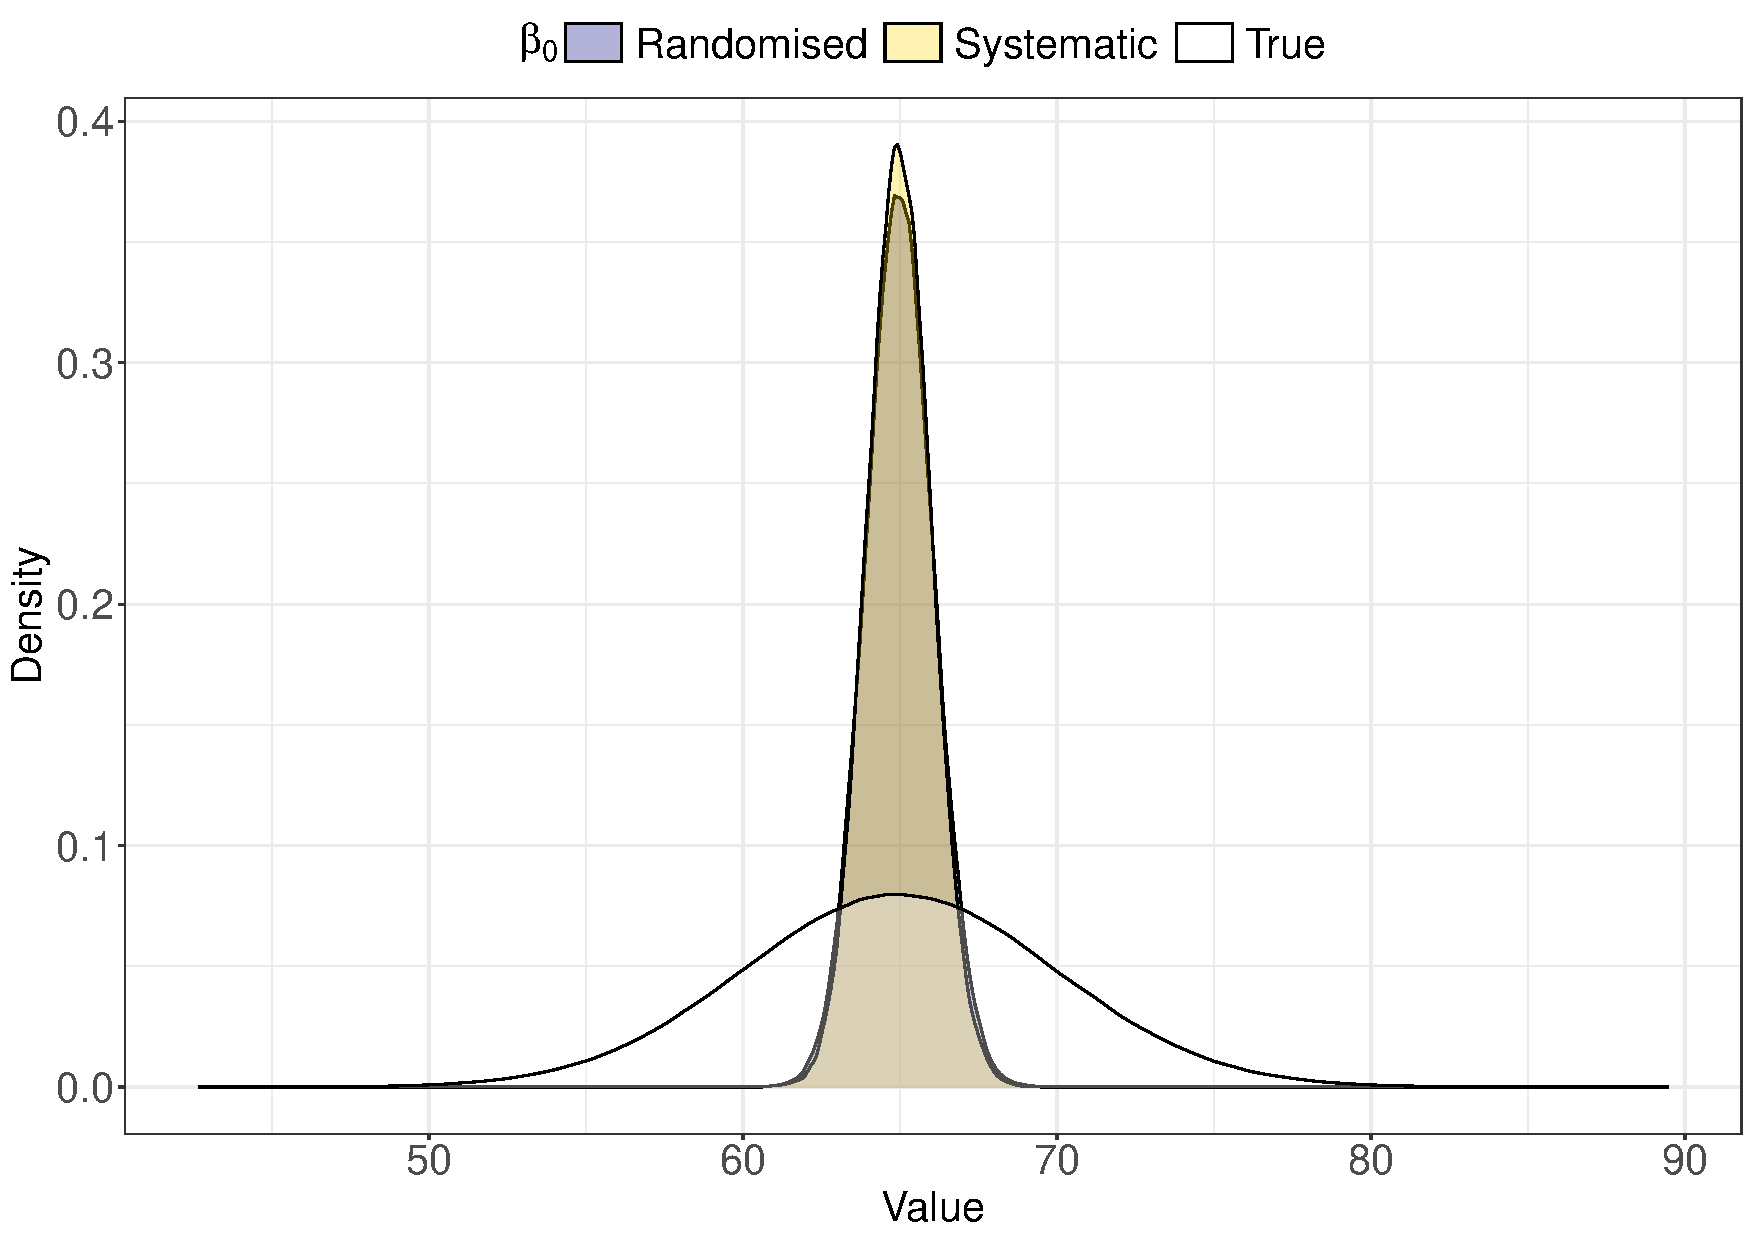
\includegraphics[width=\textwidth]{density_mat_1k_b0.pdf}
        %\caption{Plot 1}
        \label{fig:beta0_mat}
    \end{subfigure}
    \hfill
    \begin{subfigure}[b]{0.32\textwidth}
        \centering
        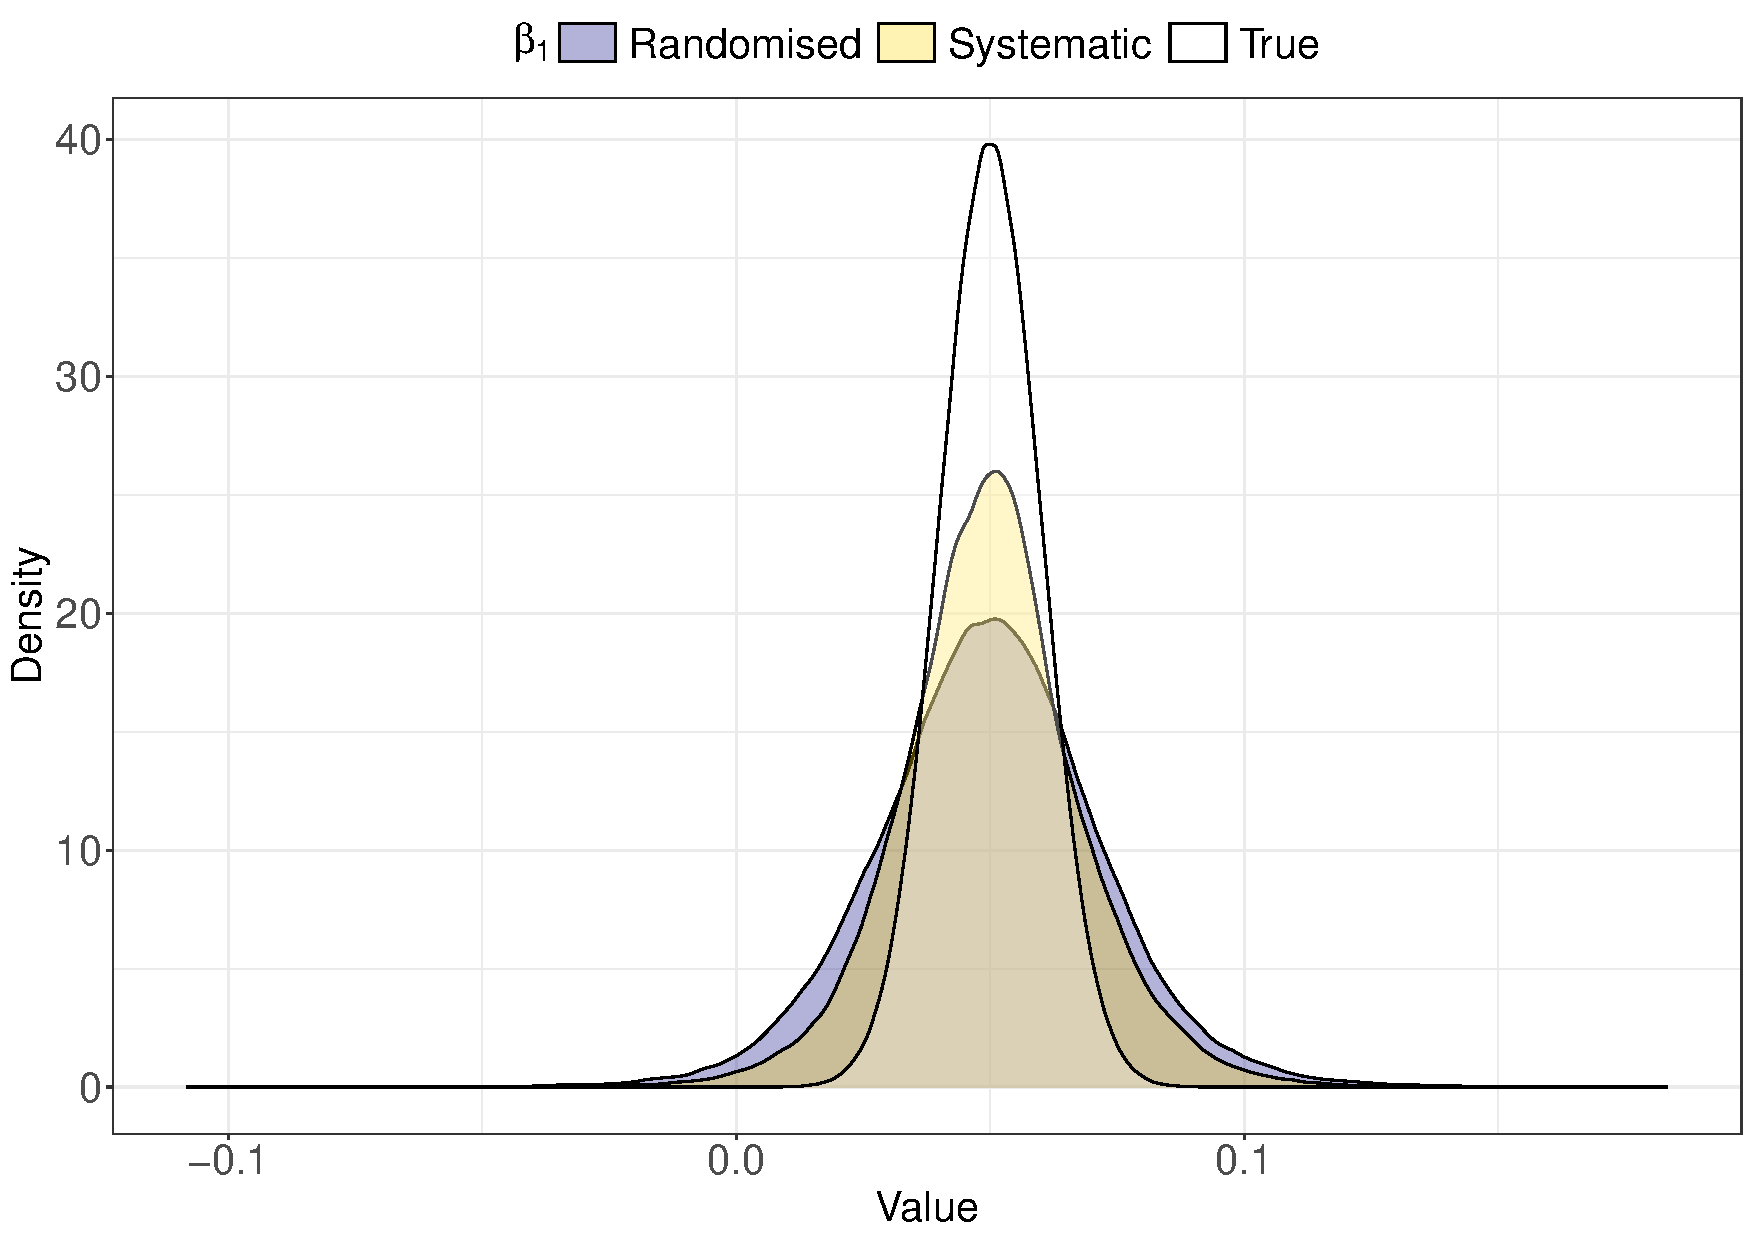
\includegraphics[width=\textwidth]{density_mat_1k_b1.pdf}
        %\caption{Plot 2}
        \label{fig:beta1_mat}
    \end{subfigure}
    \hfill
    \begin{subfigure}[b]{0.32\textwidth}
        \centering
        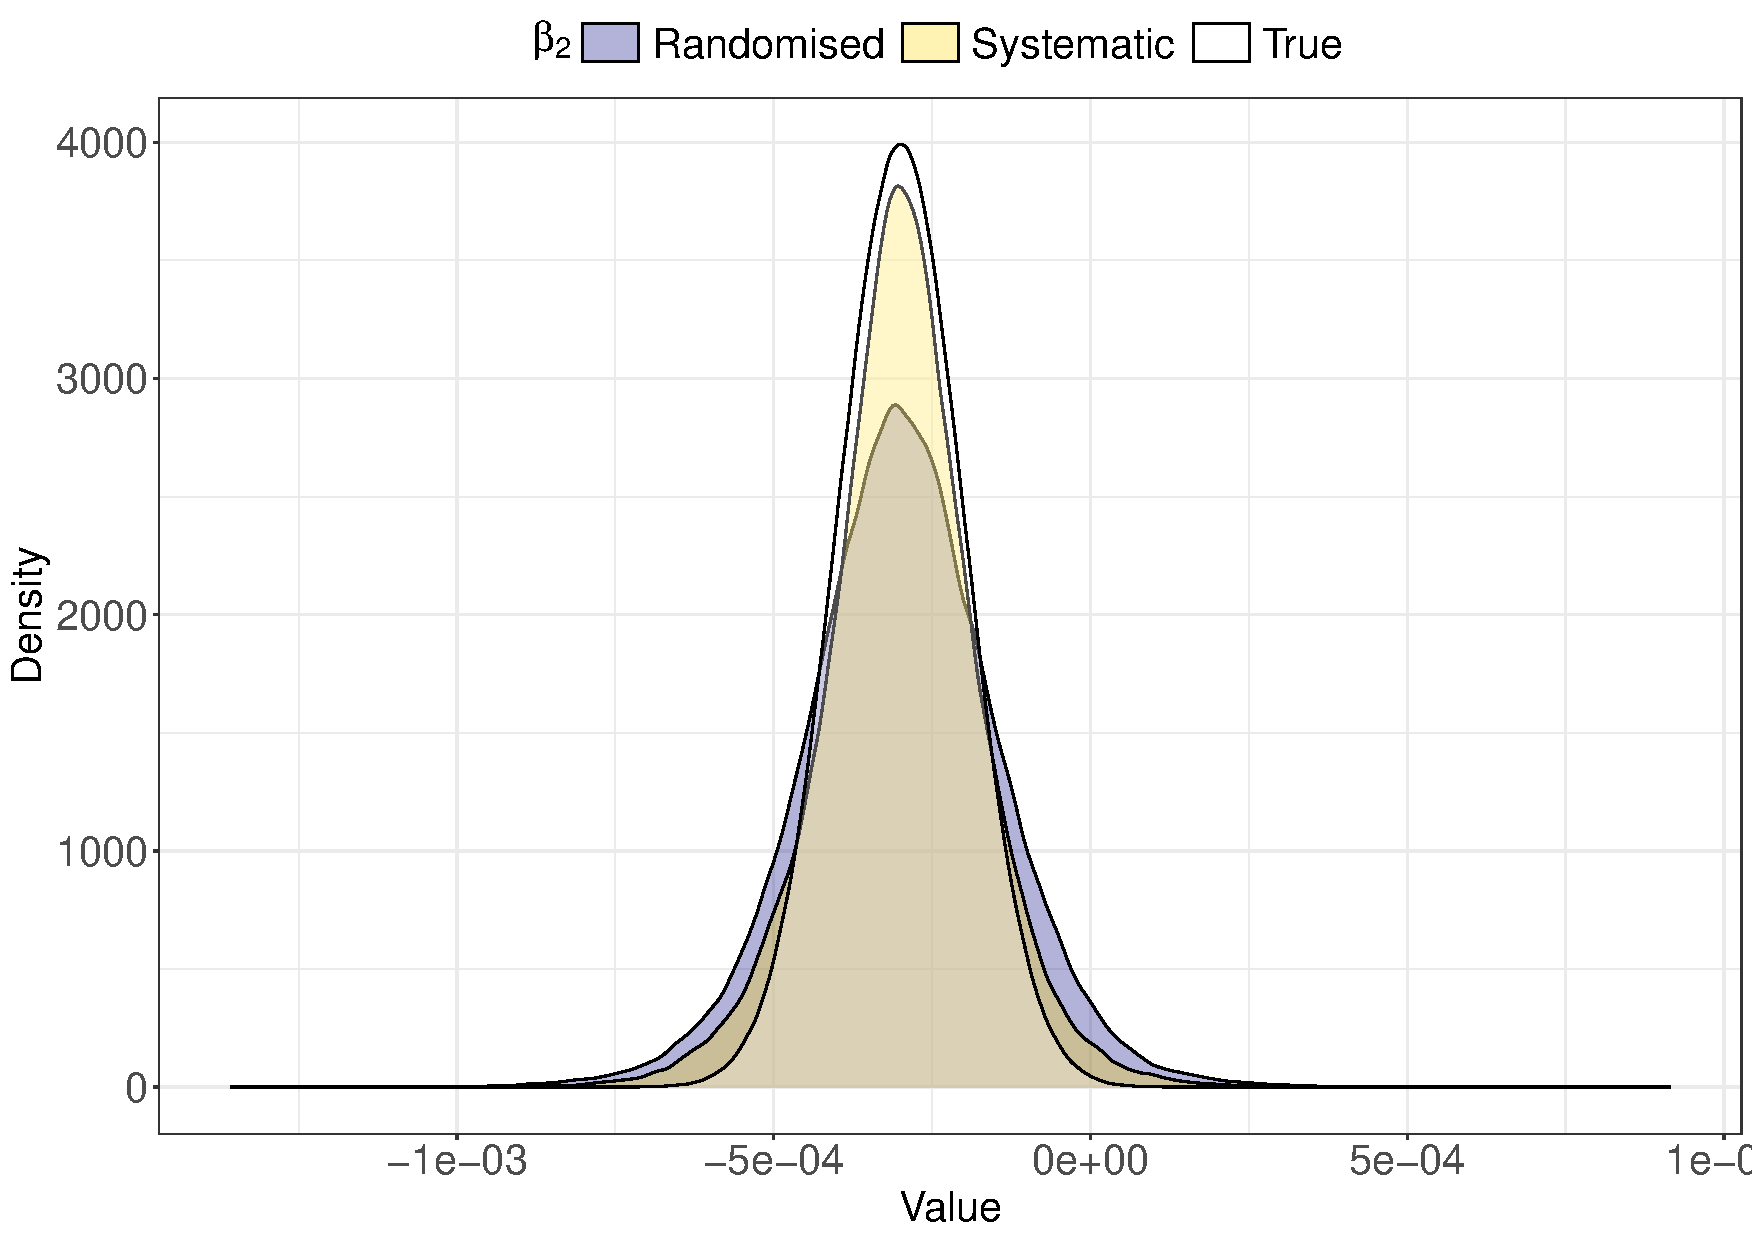
\includegraphics[width=\textwidth]{density_mat_1k_b2.pdf}
        %\caption{Plot 3}
        \label{fig:beta2_mat}
    \end{subfigure}
    \caption{\zc{Density plots comparing the true coefficients of $\beta_0$ (left), $\beta_1$ (middle), and $\beta_2$ (right) with their estimates from GWR with bandwidth 9, based on 1000 simulations.}}
    \label{fig:combinedbeta_mat}
\end{figure}






% \subsection{ANOVA}\label{Sec:anova}

% \revision{The analysis of variance (ANOVA) was used to investigate whether the differences in the results for the two designs are statistically significant and to identify the main simulation factors contributing to these differences} \zc{of the coefficients}. The analyses were performed separately for \zc{each coefficient} the two \revision{response models}. The \revision{main effects of simulation factors considered in the ANOVA models include} two designs, three bandwidths, three covariance matrices, and \zc{two types of spatial} correlation. \revision{We have also included all the second-order interactions in the ANOVA models}. The \revision{ANOVA} results are \revision{presented below} in Table~\ref{tb:LMMoutput}. 

% \zc{The ANOVA results indicate that the main effects of design, bandwidth, and covariance are highly significant in both the linear and quadratic models at the 5\% significance level.} 
% \st{The ANOVA results are consistent with what was observed in the previous subsection. For the linear response, the difference between the randomised and systematic design is not statistically significant at the 5\% significance level. In contrast, for the quadratic response model, the difference in simulation results due to different designs is statistically significant ($p$-value = 0.0177) at the 5\% significance level.}
% \zc{Bandwidth selection and covariance are all significant factors influencing the difference in results between the two design types. It is recommended that the bandwidth should be selected according to the trial design. Interestingly, the correlation within each grid is not an important factor for linear response. The interaction between design and bandwidth is significant in the quadratic response but not in the linear response. The interaction between bandwidth and covariance is significant in both response assumptions. These results suggest that bandwidth and covariance are crucial factors influencing GWR, with significant interaction effects.}

% % \begin{table}[!htp]
% % \centering
% % \caption{\zc{ANOVA results for the two response models showing the statisical significances of main effects and second-order interactions. Values reported are degrees of freedom (Df), the sum of squared errors (Sum Sq), and p-values of F tests (Pr($>$F)).}}\label{tb:LMMoutput}
% % \begin{tabular}{r | lll | lll} \toprule
% % 		& \multicolumn{3}{c|}{Linear}  & \multicolumn{3}{c}{Quadratic}  \\
% % 	  & Df & Sum Sq & Pr($>$F) & Df & Sum Sq & Pr($>$F) \\ \midrule
% % Design                       & 1  & 50     & 0.541 & 1  & 756   & 0.0177 \\ 
% % Bandwidth                    & 2  & 72446  & $<0.001$ & 2  & 882   & 0.0377 \\ 
% % Covariance ($V_s$)           & 2  & 167132 & $<0.001$ & 2  & 63668 & $<0.001$ \\ 
% % Correlation ($\epsilon$)     & 1  & 16     & 0.729 & 1  & 9     & 0.8015 \\ 
% % Design$\times$Bandwidth      & 2  & 46     & 0.841 & 2  & 1232  & 0.0103  \\ 
% % Design$\times$Covariance ($V_s$)& 2  & 27     & 0.903 & 2  & 404   & 0.2224 \\ 
% % Bandwidth$\times$Covariance ($V_s$)  & 4  & 120500 & $<0.001$ & 4  & 36174 & $<0.001$ \\ 
% % Design$\times$Correlation ($\epsilon$) & 1  & 1     & 0.918 & 1  & 68    & 0.4777 \\ 
% % Bandwidth$\times$Correlation ($\epsilon$) & 2  & 1     & 0.995 & 2  & 74    & 0.7604 \\ 
% % Covariance ($V_s$)$\times$Correlation ($\epsilon$)   & 2  & 34     & 0.881 & 2  & 23    & 0.9181 \\ 
% % \bottomrule
% % \end{tabular}
% % \end{table}


% \begin{table}[!htp]
% \centering
% \caption{\zc{ANOVA results for the two response models showing the statisical significances of main effects and second-order interactions. Values reported are degrees of freedom (Df), the sum of squared errors (Sum Sq), and p-values of F tests (Pr($>$F)).}}\label{tb:LMMoutput}
% \resizebox{\textwidth}{!}{%
% \begin{tabular}{r|lll|lll|lll} \toprule
%  & \multicolumn{3}{c|}{Linear $\beta_1$} & \multicolumn{3}{c}{Quadratic $\beta_1$} & \multicolumn{3}{c}{Quadratic $\beta_2$}   \\ 
%  & Df  & Sum Sq  ($\times 10^{6}$)  & Pr($>$F)  & Df   & Sum Sq   & Pr($>$F)& Df & Sum Sq ($\times 10^{12}$)   & Pr($>$F)\\ \midrule
% Design& 1   & 3.2 & $<0.001$  & 1& 0.0016   & $<0.001$  & 1  & 4 & $<0.001$ \\
% Bandwidth   & 2   & 2441.8 & $<0.001$  & 2& 0.4151   & $<0.001$  & 2  & 907 & $<0.001$ \\
% Covariance ($V_s$)  & 2   & 914.4 & $<0.001$  & 2& 0.1487   & $<0.001$   & 2  & 332 & $<0.001$ \\
% Correlation ($\epsilon$)  & 1   & $<0.1$ & 0.561& 1& 0.0001   & $<0.001$& 1  & 1 & $<0.001$  \\
% Design$\times$Bandwidth & 2   & 2.6 & $<0.001$  & 2& 0.0020   & $<0.001$   & 2  & 4.5 & $<0.001$ \\
% Design$\times$Covariance ($V_s$)& 2   & 1.8 & $<0.001$  & 2& 0.0008   & $<0.001$  & 2  & 2 & $<0.001$ \\
% Design$\times$Correlation ($\epsilon$)& 1   & 1 & 0.284& 1& 0.0001   & $<0.001$  & 1  & 0.1 & 0.025 \\
% Bandwidth$\times$Covariance ($V_s$) & 4   & 1405.3 & $<0.001$  & 4& 0.2293   & $<0.001$  & 4  & 507 & $<0.001$ \\
% Bandwidth$\times$Correlation ($\epsilon$) & 2   & $<0.1$ & 0.986& 2& 0.0002   & $<0.001$  & 2  & 1.70 & $<0.001$ \\
% Covariance ($V_s$)$\times$Correlation ($\epsilon$)& 2   & 0.3 & 0.082& 2& 0.0001   & 0.011 & 2  & 0.9 & $<0.001$   \\ \bottomrule
% \end{tabular}
% }
% \end{table}



% \zc{In designing an OFE trial, it is crucial to consider the types of trial design and the covariance matrix depending on the purpose of the experiment. Furthermore, when fitting the GWR model to OFE trial data, the bandwidth selection is a key factor that requires careful consideration.}


\subsection{\zc{An example of optimal nitrogen map}}


\zc{In practice, growers are more interested in the prescription map that tells them where the appropriate nitrogen should be applied on the paddock. With the application of GWR, we can find the local variations in crop needs, allowing for more precise and efficient nitrogen application. Each grid of the paddock receives the optimal amount of fertiliser. Consequently, this leads to improved crop yields, reduced investment cost and high profit.}


\zc{Figure \ref{fig:yieldmap} is the simulated crop yield map with the assumption of a quadratic response curve and \Matern spatial covariance and low within-grid correlation. These two yield maps have the same coefficients but different yields due to different treatment layouts.}

\begin{figure}[!htp]
\centering
    \begin{subfigure}[t]{0.9\textwidth}
		\centering
		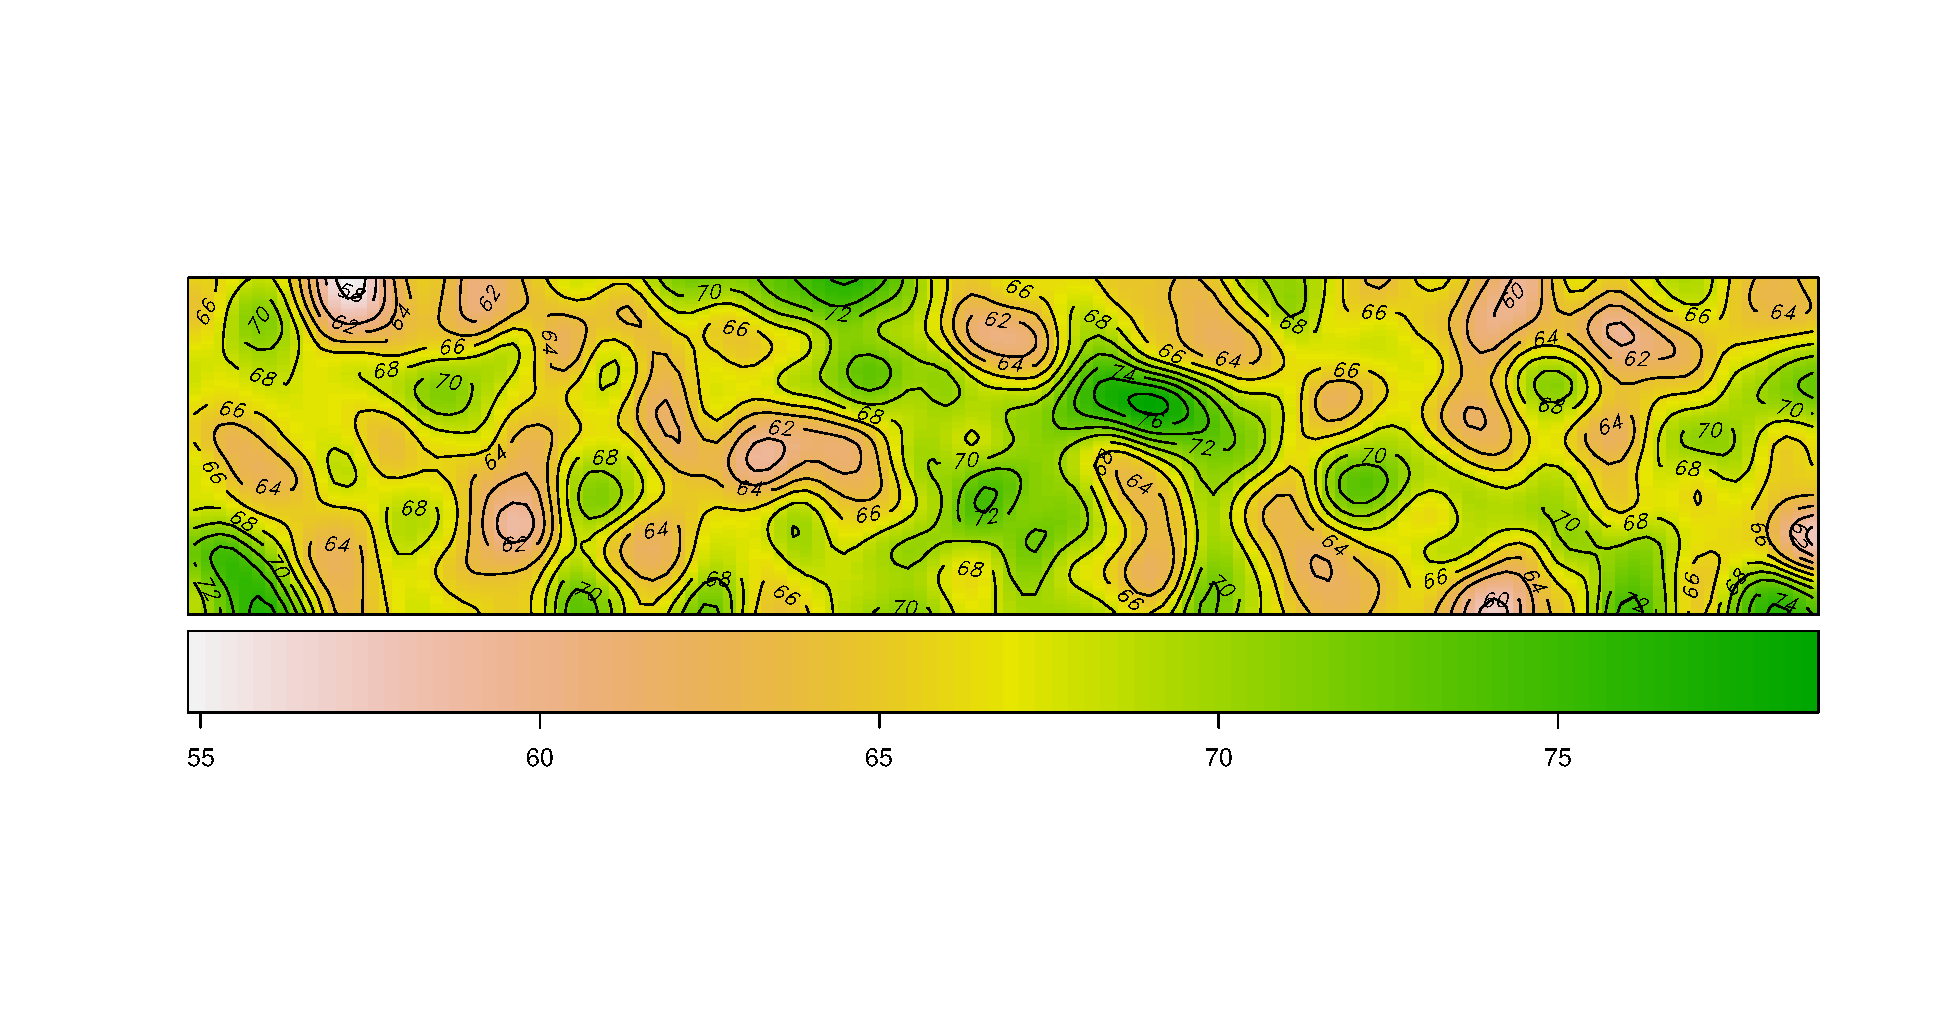
\includegraphics[width=\linewidth]{quad_random_yield_mat.pdf}
		%\caption{}
    \end{subfigure}
    %\hspace{0.05\textwidth}
    \begin{subfigure}[t]{0.9\textwidth}
		\centering
		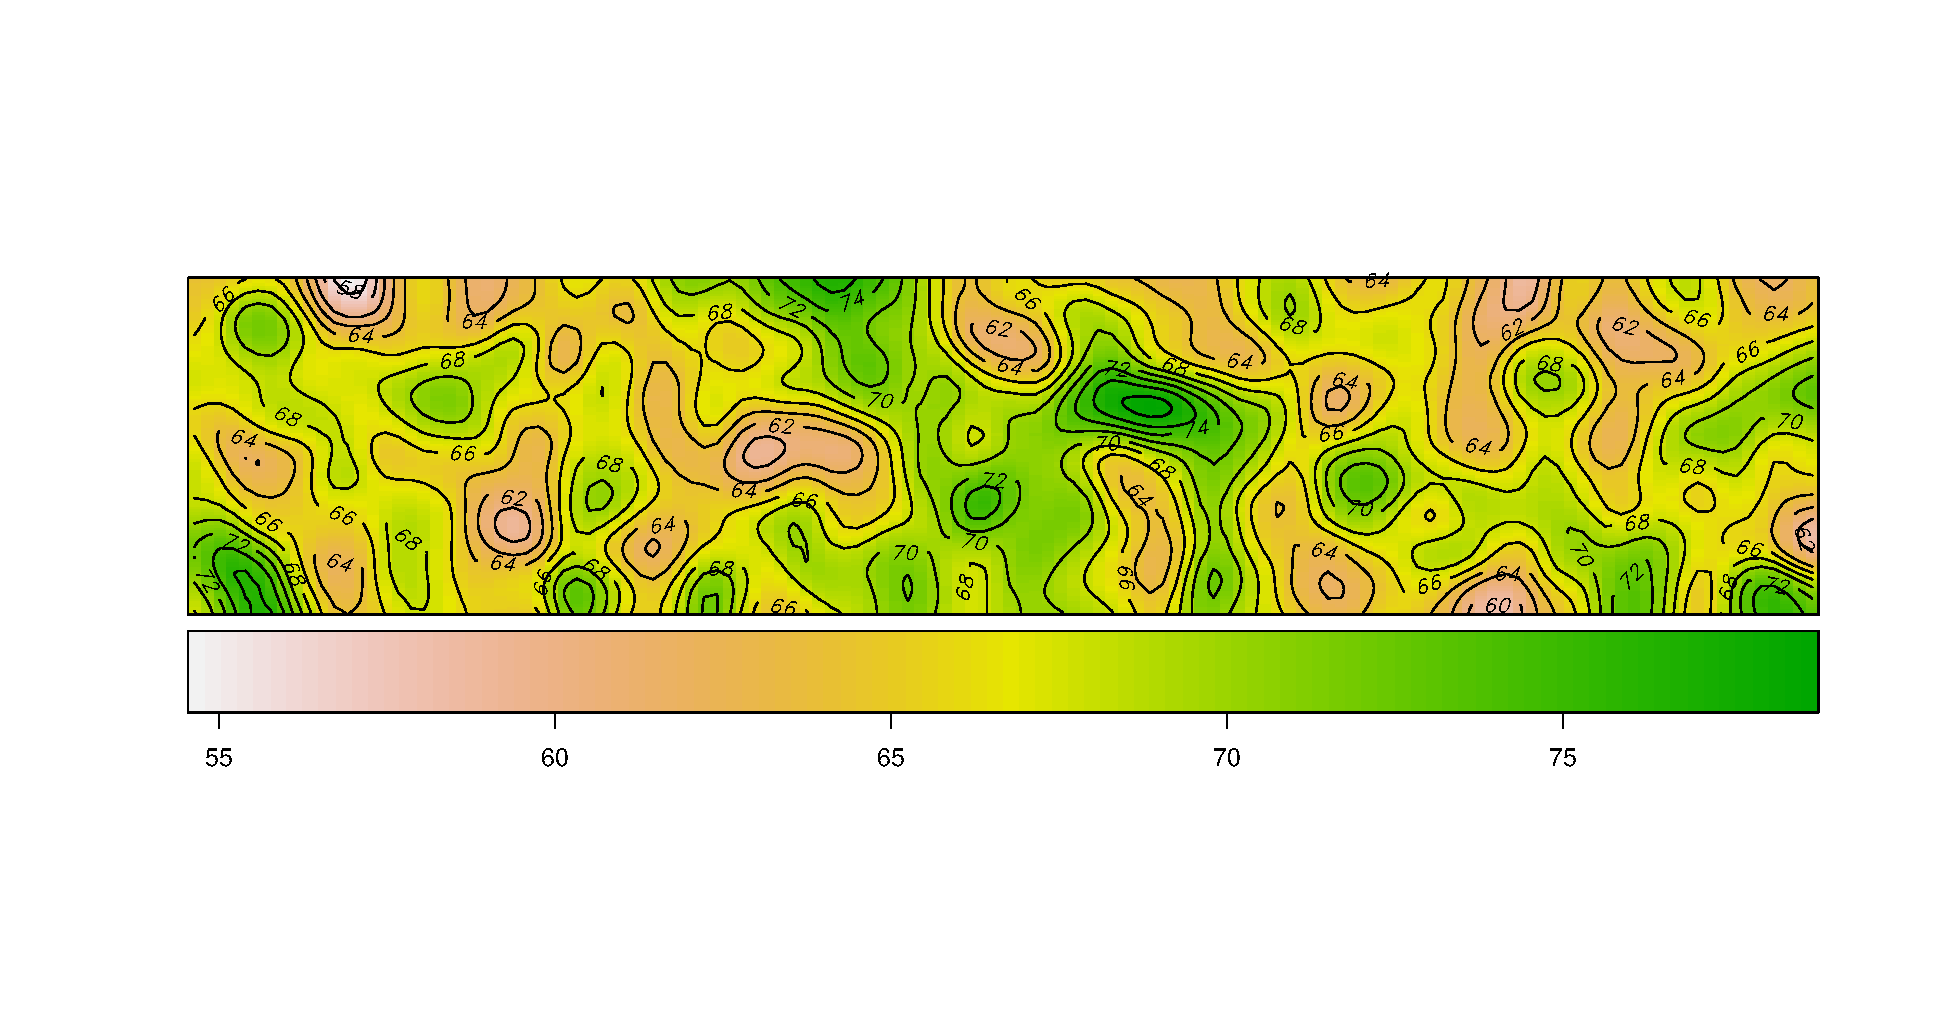
\includegraphics[width=\linewidth]{quad_syst_yield_mat.pdf}
		%\caption{}
    \end{subfigure}
    \begin{subfigure}[t]{0.9\textwidth}
		\centering
		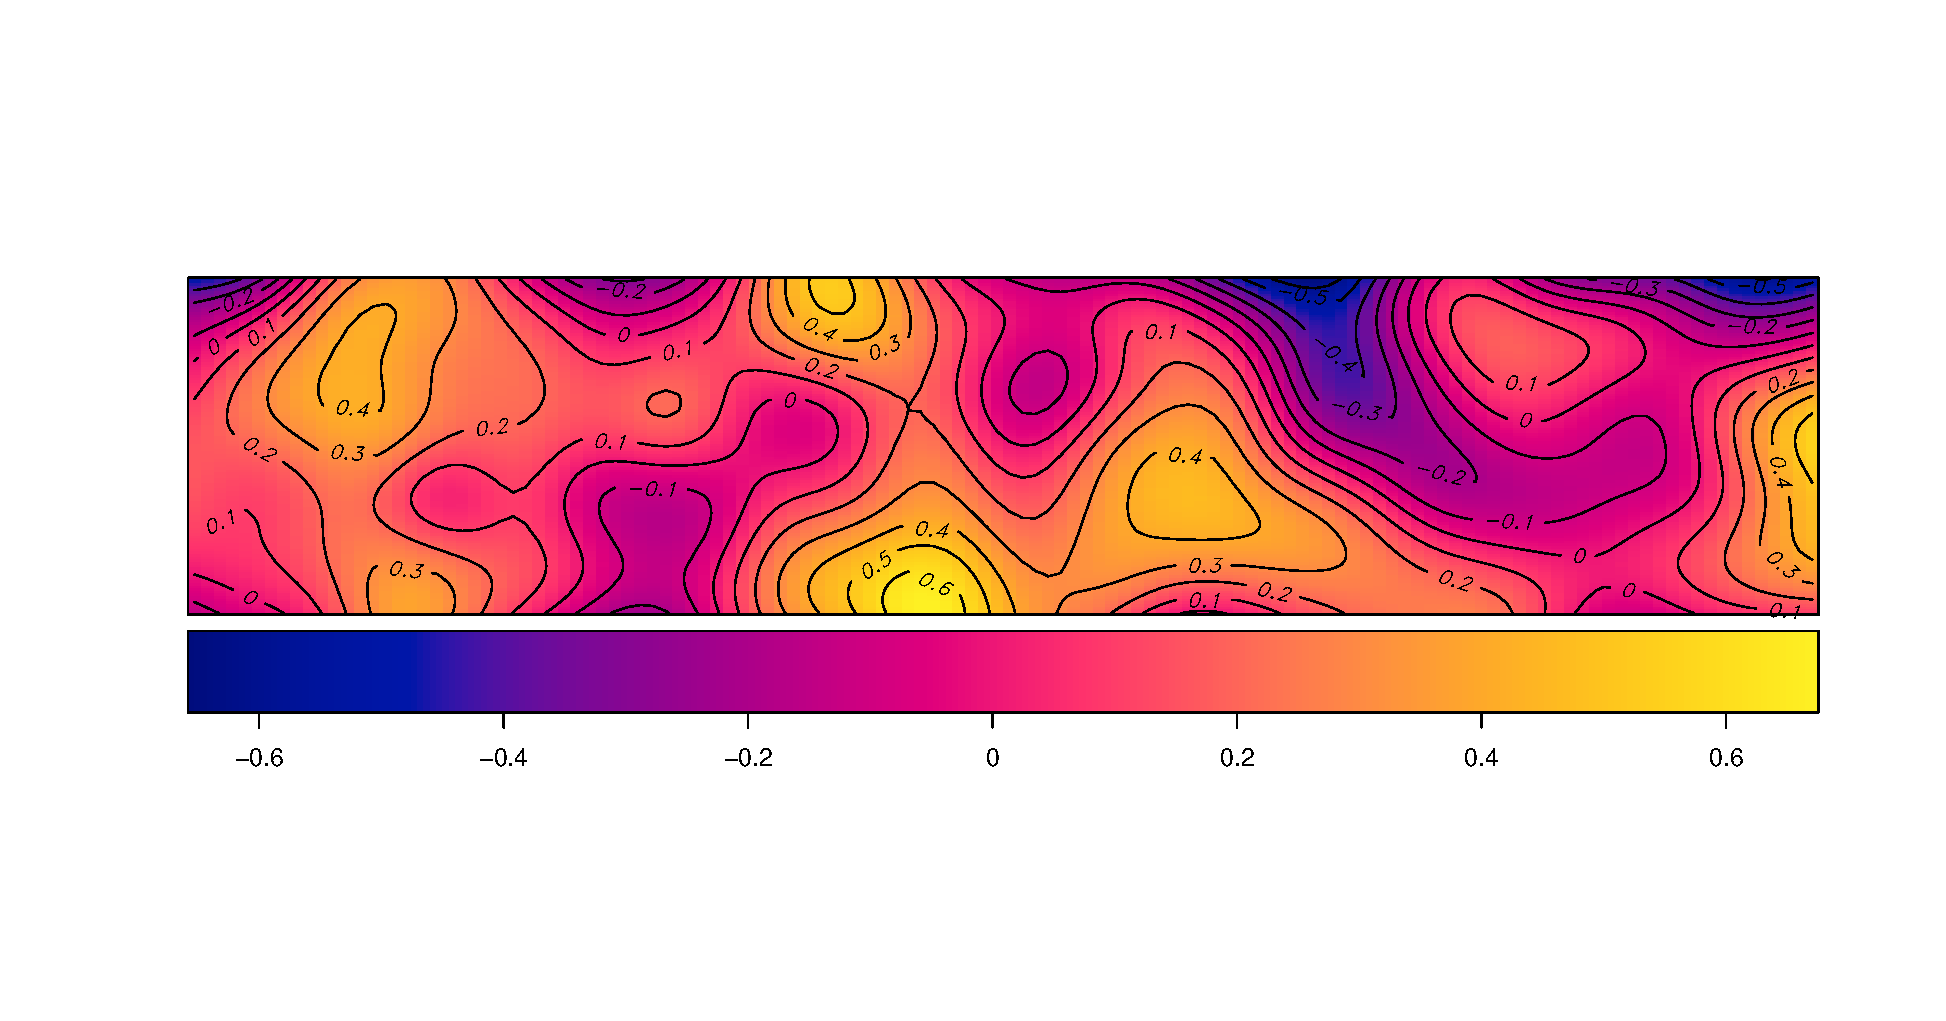
\includegraphics[width=\linewidth]{quad_diff_yield_mat.pdf}
		%\caption{}
    \end{subfigure}
	\caption{\zc{Simulated yield map of a randomised design (\textit{top}), and a systematic design (\textit{middle}), and the difference of these two designs (\textit{bottom}).}}\label{fig:yieldmap}
\end{figure}


\zc{Figure \ref{fig:optNmap} illustrates an example of the optimal Nitrogen rate (kg/ha) map estimated by GWR with a bandwidth of 9 using the above yield data. The optimal rate at grid $i$ is given by $\hat{N}_i = -\hat{\beta}_{1i}/(2\hat{\beta}_{2i})$ with constraints between 0 and 140, $i=1,\ldots,n$. For the randomised design, GWR underestimated the right part of the paddock. On the contrary, the estimated map from the systematic design is more consistent.}

\begin{figure}[!htp]
	\begin{subfigure}[t]{0.45\textwidth}
		\centering
		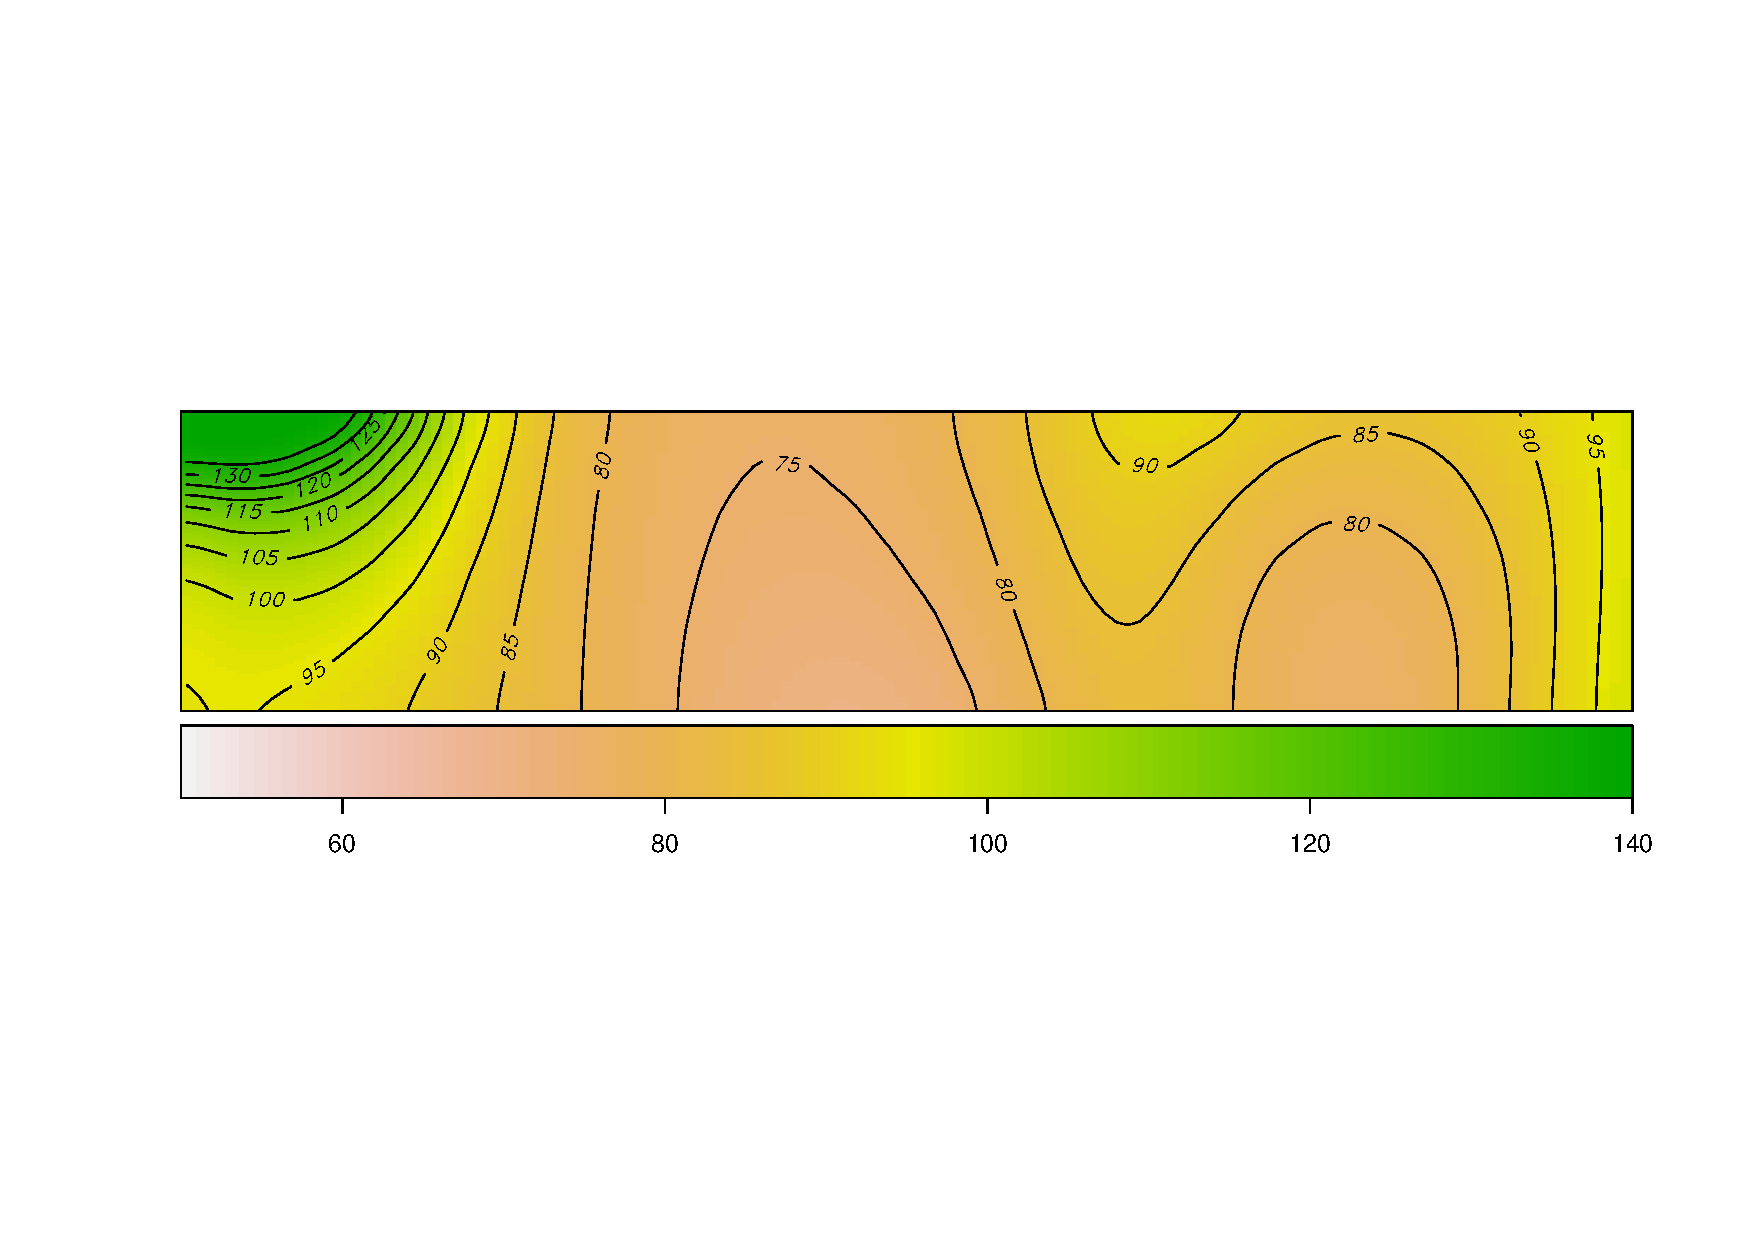
\includegraphics[width=\linewidth]{optN_rand_matB9.pdf}
		%\caption{}
 \end{subfigure}
	\hspace{0.05\textwidth}
	\begin{subfigure}[t]{0.45\textwidth}
		\centering
		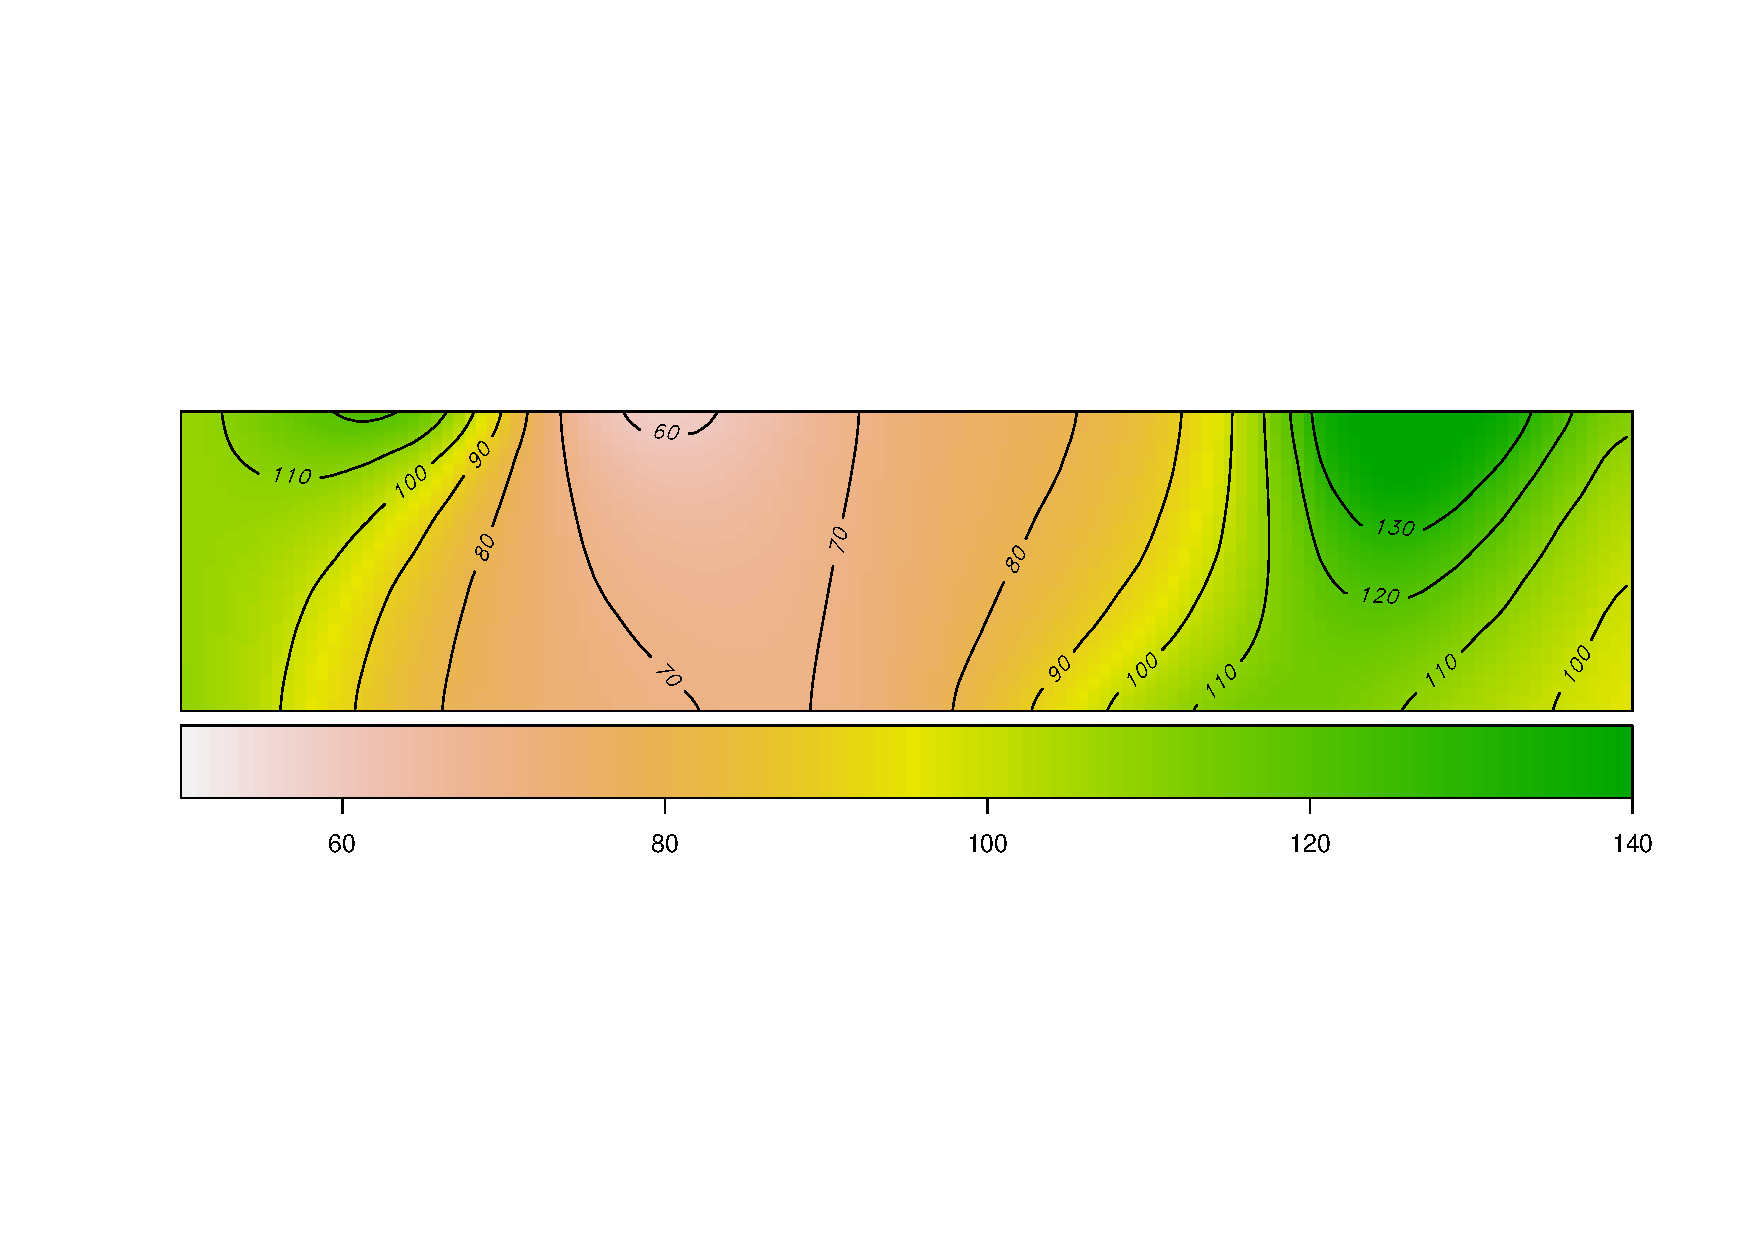
\includegraphics[width=\linewidth]{optN_syst_matB9.pdf}
		%\caption{}
 \end{subfigure}
	\caption{\zc{Optimal Nitrogen rate estimated by GWR from a randomised design (\textit{left}), and a systematic design (\textit{right}).}}\label{fig:optNmap}
\end{figure}


\section{Discussion}\label{Sec:Dis}

%1. Summary of Main Findings
Agronomists and biometricians generally prefer randomised designs for OFE trials. \zc{This is likely due to their experience with small-plot field experiments, where randomised designs are employed.} \zc{O}ur simulation study shows a systematic design performs either preferably or similarly to a randomised design for the purposes of creating a varying treatment map \zc{when using the performance metrics stated}. The differentiating factors \zc{primarily included} the response type and the spatial covariance model, while the correlation amongst the treatment coefficients \zc{is} not found to be important. These are factors that can be assessed by the farmer \zc{and their agronomists} beforehand, and this should dictate which design should be used. \zc{G}iven that a systematic design is easier to implement in the field, and shows little downside to \zc{creating} a varying treatment map, the use of systematic designs \zc{is recommended}. 

%2. How response type affected the performance, and what this means
The response type \zc{is} the main differentiating factor between randomised and systematic designs. When the response \zc{is} quadratic, the systematic design performed favourably, \zc{contrasting with} the result \zc{of} the linear design. Given this, if an approximately linear response \zc{is expected} in the field, then the selection of the design may not be important. However, given the variable nature of the relationship between response and treatment over a large field (see \textcite{Rakshit2020Novel}), it may be wise to implement a systematic design for the potential outcome of a quadratic relationship. 
%For other more complex response types (i.e polynomials of order greater than 2) it is predicted that a systematic design will also perform favourably. \textcolor{red}{?ref}
%(\textcolor{red}{Might not need a reference)}. 

%2. Discussing Spatial Covariance Structures
%- Some Questions that might be interesting to answer
%- Is a \Matern class more realistic and what are its limitations? %- 

Another consideration for \zc{agronomists and biometricians when selecting} which design to use is the expected spatial covariance structure in the field. When no spatial structure was simulated, the differences between the prediction from the systematic and random design \zc{are} minimal. This result should be expected given that if there are no spatial autocorrelations, then the individual query grids are independent observations, and therefore the design is not important. However, when a first-order auto-regressive structure was simulated, the differences \zc{are} noticeable when a quadratic response was used, showing systematic designs to be preferential. The largest difference between the two designs occurred when considering the \Matern spatial covariance structure, which showed a clear preference for systematic designs when a quadratic response was considered, and also a small preference for systematic designs for a linear response. Therefore, only if spatial variability \zc{is} predicted to be negligible in the field would using a randomised design be reasonable given a quadratic response. This assumption of negligible spatial variability would be difficult to reason with given the large fields used in on-farm experimentation, meaning that in the application a systematic design should be used. 

% Spatial stationarity is seldom the case in small plot research trials even in highly controlled environments. 

%3. Bandwidth selection and why that is important [good]
There \zc{are} significant deficiencies \zc{found} in using AICc for bandwidth selection. The AICc-\zc{selected} bandwidths skewed to 1 and, in a few cases, ended in 93 (number of rows). Even though the bandwidth \zc{is} optimal according to AICc, the MSE \zc{is} higher than when using a fixed bandwidth. Therefore, a fixed bandwidth based on the experimental design (5 or 9 in this case) \zc{is recommended}, rather than \zc{AICc-selected bandwidth}. Selecting the bandwidth based on the experimental design is also theoretically better since \zc{when} only a single measurement is observed in each grid, all levels of the treatment factor should be included in a GWR window at the same time to interpolate the relationship. \zc{If more than one level is missing, then the interpolation is incomplete.} 


\zc{Our study employs simulation to evaluate the effectiveness of GWR in estimating coefficients for both randomised and systematic designs. However, a potential drawback of using simulation is its high dependency on the assumptions underlying the parametric model. If these assumptions are incorrect or fail to accurately represent real-world conditions, the simulation results may not reliably reflect the actual scenario.}

% ... AICc-minimising bandwidth were skewed towards the upper ($sqrt(19^2+92^2)=93.94147$) or lower (1) bounds; two characteristics which are suggestive of underlying stationary or random processes  respectively \textcite{}.  
% In this paper, the simulated data is fitted by GWR, which has been proven to accurately separate treatment from non-treatment influence of yield response. One crucial factor of GWR is bandwidth selection. The AICc-minimising bandwidths skew to 1 and, in a few cases, end in 93 (number of rows). Thus, even though the bandwidth is optimal, the MSE is higher than when using a fixed bandwidth. Therefore, we would use the fixed bandwidth of 5 and 9 based on the experimental design, rather than the recommended bandwidth from AICc. Selecting the bandwidth based on the experimental design is also theoretically better. Since only a single measurement is observed in each grid, all levels of the treatment factor should be included in a GWR window at the same time to interpolate the quadratic curve. Otherwise, the interpolation is incomplete if more than one level is missing. 

%4. Paragraph on Coefficient importance (or the lack thereof)
%The level of correlation between the coefficients as governed by $\epsilon$ was found to no be significant (Table \ref{tb:LMMoutput}). This indicates that GWR performs similarly with either low or high correlation between coefficients. %This is an unexpected/expected result... 

%5. Recommendation of design variations
Given the scope of the paper, some designs and factors were not considered. Designs such as chequerboard or wave designs have been suggested for on-farm experiments \parencite{bramley1999designing}, however, were not considered here. Topographical factors (spatial zones) were also not entertained in our study. Since GWR estimates a global template model and then adjusts it at a local scale across the study region, the variation between zones is ``flushed out'' by the spatial covariance.

%However, this is not practical for farmers as the complex layout of the treatments will increase the cost of sowing and harvesting. Therefore, unless the objective is for variety selection, we do not recommend such designs to agronomists. 

%6. Recommendation of other spatial factors to consider, and why those were ignored. 
%Topographical factors (spatial zones) were also not considered in our study. Since GWR estimates a global template model and then adjusts it at a local scale across the study region, the variation between zones is ``flushed out'' by the spatial covariance.

\section{Conclusion}\label{Sec:Conclusion}

% Agronomists and biometricians generally prefer randomised designs for OFE trials. With the purpose of creating a varying treatment map, our simulation study proves that a systematic design produces better performance metrics, under particular circumstances, than a randomised design for large on-farm trials in terms of robustness and smaller MSE on coefficients. On the other hand, if spatial variation is not considered or if researchers believe in linear response, a systematic or a randomised design could be implemented because the difference is not significant. We recommend that, for a large OFE strip trial with the goal to create a varying treatment map, a systemic design should be used as it has more flexibility in post-experiment statistical modelling. 


\zc{This research offers a number of recommendations for agronomists and biometricians for designing OFE trials.}
\zc{
\begin{itemize}
    \item Systematic designs are suitable for OFE trials, particularly when the results will be used to develop a variable rate map for the treatment, such as fertiliser. 
    \item Incorporation of a quadratic function for GWR is preferred for systematic designs when spatial variability is present.
    \item Using a fixed bandwidth for GWR analysis based on experimental design, such as the number of treatments. 
\end{itemize}
}
% Perhaps we add a comment along the lines - "Further research is needed in the case of OFE (and GWR?) when it comes to more complex designs such as chequerboard, donut etc."

\section*{Acknowledgements}

Curtin Biometry and \zc{Agricultural} Data Analytics (CBADA) gratefully acknowledges the support from the Grains Research and Development Corporation of Australia (GRDC).

\section*{CRediT authorship contribution statement}

\textbf{Zhanglong Cao}: Conceptualization; Formal analysis; Methodology; Software; Validation; Visualization; Roles/ Writing - original draft; and Writing - review \& editing. \textbf{Jordan Brown}: Investigation; Methodology; Visualization; Roles/Writing - original draft; and Writing - review \& editing. \textbf{Mark Gibberd}: Project administration; Roles/Writing - original draft; and Writing - review \& editing. \textbf{Julia Easton}: Roles/Writing - original draft; and Writing - review \& editing. \textbf{Suman Rakshit}: Conceptualization; Methodology; Supervision; Roles/Writing - original draft; and Writing - review \& editing. 


\renewcommand\bibname{References}% change bibliography title to references
	%\addcontentsline{toc}{chapter}{Bibliography}
\addtocontents{toc}{Bibliography}
\printbibliography
\end{document}
